\documentclass[10pt]{beamer}


% colors
\usepackage{xcolor}
\definecolor{mydarkgray}{gray}{0.33}
\definecolor{myred}{rgb}{0.85, 0.30, 0.0}
\definecolor{myblue}{rgb}{0.01, 0.45, 0.70}
\definecolor{mylightgray}{gray}{0.5}
\definecolor{mylightestgray}{gray}{0.9}


% beamer options
\setbeamertemplate{caption}[numbered]
\setbeamertemplate{frametitle}[default][center]
\setbeamertemplate{itemize items}[circle]
\setbeamertemplate{itemize subitem}{$\circ$}

\setbeamercolor{title}{fg=myblue}
\setbeamercolor{titlelike}{fg=mydarkgray}
\setbeamercolor{frametitle}{fg=mydarkgray, bg=mylightestgray}
\setbeamercolor{framesubtitle}{fg=mylightgray}
\setbeamercolor{itemize item}{fg=mydarkgray}
\setbeamercolor{itemize subitem}{fg=mydarkgray}


% figures
\usepackage{graphicx}


% language
\usepackage[english]{babel}
\usepackage[utf8]{inputenc}
\usepackage[T1]{fontenc}
\usepackage{biblatex}
\addbibresource{reports/paper/refs.bib}
% titlepage
\author{Xiao Chen, Bosko Todorovic, Yannic Laube, Zhi Wang}

\title{Which of the G10 Currencies is the Riskiest to Hold for a Swiss Resident?}

\institute{University of Zurich}
\date{\today}

\begin{document}
% ---------------------------------------------------------------------------
\begin{frame}
\titlepage
\end{frame}
% ---------------------------------------------------------------------------
\begin{frame}
\frametitle{Table of Contents}
\tableofcontents
\end{frame}
% ---------------------------------------------------------------------------
\begin{frame}
\section{Introduction}
\frametitle{Introduction}
\framesubtitle{G10 currencies}
G10 currencies refer to the ten most heavily traded and liquid currencies in the world: 

United States Dollar (USD), Euro (EUR), British Pound (GBP), Japanese Yen (JPY), Australian Dollar (AUD), New Zealand Dollar (NZD), Canadian Dollar (CAD), Swiss Franc (CHF), Norwegian Krone (NOK), and Swedish Krona (SEK).

\end{frame}
% ---------------------------------------------------------------------------
\begin{frame}
\frametitle{Introduction}
\framesubtitle{G10 currencies}
Swiss residents holding assets denominated in other G10
currencies still face potential risks arising from exchange rate fluctuations:
\begin{itemize}
    \item Asset value depreciation
    \item Increased transaction costs
    \item Financial market volatility affecting their investment portfolios
\end{itemize}

G10 currencies also play a critical role in various aspects of Swiss residents’ financial activities.
\end{frame}
% ---------------------------------------------------------------------------
\begin{frame}
\section{Literature Review}
\frametitle{Literature Review}
Relationship between exchange rate fluctuations, international trade, and cross-border investments:~\cite{AUBOIN_RUTA_2013}
\begin{itemize}
    \item Exchange rate volatility introduces uncertainties for exporters and importers.
    \item Companies experiencing sharp exchange rate fluctuations may experience revenue shrinkage.
\end{itemize}
\end{frame}
% ---------------------------------------------------------------------------
\begin{frame}
\frametitle{Literature Review}
Persistent exchange rate changes influence strategic decisions of multinational corporations, including investment location
choices and capital allocation:~\cite{riker2020review}
\begin{itemize}
    \item U.S. dollar appreciation often reduces USD-denominated cross-border banking flows.~\cite{dollar_exchange}
    \item Imposing greater financing and investment risks on countries and corporations heavily reliant on USD debt.~\cite{dollar_exchange}
\end{itemize}
\end{frame}
% ---------------------------------------------------------------------------
\begin{frame}
\frametitle{Literature Review}
\framesubtitle{Characteristics}
\textbf{Liquidity}~\cite{rogoff2000six}
\begin{itemize}
    \item High foreign exchange trading volume
    \item Active derivatives trading
    \item Core position in foreign exchange reserves
\end{itemize}
\textbf{Stability}~\cite{campbell2002strategic}~\cite{engel2016exchange}
\begin{itemize}
    \item Strong economic foundations
    \item Safe-haven attributes
    \item Mitigate likelihood of extreme losses
\end{itemize}
\end{frame}
% ---------------------------------------------------------------------------
\begin{frame}
\frametitle{Literature Review}
\framesubtitle{Why Are G10 Currencies Important to Swiss Residents?}
\textbf{Trading and Investment}
\begin{itemize}
    \item Ease of Cross-Border Investment~\cite{rogoff2000six}: High-liquidity G10 currencies, such as the US dollar (USD), euro (EUR), and Japanese yen (JPY), make it easier for Swiss residents to participate in global investment opportunities, including equities, bonds, and real estate.
    \item Predictable Investment Returns~\cite{campbell2002strategic}~\cite{engel2016exchange}: Stable G10 currencies reduce exchange rate risks, making investment returns more predictable and reducing the risk of extreme losses.
\end{itemize}
\end{frame}
% ---------------------------------------------------------------------------
\begin{frame}
\frametitle{Literature Review}
\framesubtitle{Why Are G10 Currencies Important to Swiss Residents?}
\textbf{Saving and Payments}
\begin{itemize}
    \item Euro as a Key Currency: Switzerland is near the Euro Area, so the euro (EUR) becomes the main currency for Swiss residents in addition to the Swiss Franc. It is widely used for cross-border shopping, travel, and international payments.
\end{itemize}
\end{frame}
% ---------------------------------------------------------------------------
\begin{frame}
\frametitle{Literature Review}
\framesubtitle{Why Are G10 Currencies Important to Swiss Residents?}
\textbf{Asset Diversification and Safe-Haven Properties}   
\begin{itemize}
    \item Asset Diversification: The stability and liquidity of G10 currencies allow Swiss residents to diversify their assets beyond the Swiss franc. This is particularly relevant for mitigating risks in times of economic uncertainty.~\cite{ito2020currency}
    \item Safe-Haven Currencies: Stable currencies show strong safe haven characteristics during periods of global financial turbulence or geopolitical instability. Swiss residents can leverage these currencies to preserve wealth in uncertain times.~\cite{ranaldo2010safe}
\end{itemize}
\end{frame}
% ---------------------------------------------------------------------------
\begin{frame}
\frametitle{Research Objective}
Compare and analyze: "Which of the G10 currencies is the riskiest to hold for a Swiss resident?"
\end{frame}
% ---------------------------------------------------------------------------
\begin{frame}
\section{Methodology}
\frametitle{Methodology}
The methods used include the calculation of Expected Shortfall (ES), Value-at-Risk (VaR) through different models, the analysis of volatilities, and the investigation of the sensitivity of exchange rate returns to interest rate differentials.
\end{frame}
% ---------------------------------------------------------------------------
\begin{frame}
\frametitle{Methodology}
\framesubtitle{Expected Shortfall}

\end{frame}
% ---------------------------------------------------------------------------
\begin{frame}
\frametitle{Methodology}
\framesubtitle{Value-at-Risk (VaR)}
The loss that will not be exceeded with a certain probability and within a specified time period. 

Frequency = D (Day), $\alpha = 0.05$. 

Two different methods for calculating VaR were applied:
\begin{itemize}
    \item Historical calculation
    \item Monte Carlo simulation
\end{itemize}.

\end{frame}
% ---------------------------------------------------------------------------
\begin{frame}
\frametitle{Methodology}
\framesubtitle{Historical vs. Monte Carlo Simulation}
\begin{itemize}
    \item \textbf{Historical calculation:} Based on the empirical distribution of historical returns, and does not make any assumptions about the distribution of returns and thus reflects realistic market conditions.
    \item \textbf{Monte Carlo simulation:} 10 simulations were conducted. The VaR for the simulated price paths and simulated returns was calculated for the last period of the simulation, and the VaR was explicitly visualized in the return simulation. 
\end{itemize}
\end{frame}
% ---------------------------------------------------------------------------
\begin{frame}
\frametitle{Methodology}
\framesubtitle{Volatility Analysis}
\begin{itemize}
    \item Volatility was calculated as a measure of the fluctuation intensity of the exchange rates. It was determined based on the standard deviation of the daily returns. High volatility values indicate increased risk, as larger fluctuations in exchange rates imply higher uncertainties.
    \item The volatilities of the G10 currencies were compared to identify which currency poses the greatest risk for a Swiss investor.
    \item Time series plots were created to visualize volatility trends during the study period.
\end{itemize}
\end{frame}
% ---------------------------------------------------------------------------
\begin{frame}
\frametitle{Methodology}
\framesubtitle{Interest Rate Differentials Regression}
\begin{itemize}
    \item The sensitivity of exchange rate returns to interest rate differentials was examined using linear regression analysis. 
    \item Regression model: \[
    \text{log\_return}_{\text{exchange}} = \alpha + \beta \cdot \text{log\_diff}_{\text{interest\_rate}} + \epsilon
    \]
    \item Significance tests and confidence intervals were used to assess the statistical significance of the parameters. A detailed summary of the regression was created for each currency.
\end{itemize}
\end{frame}
% ---------------------------------------------------------------------------
\begin{frame}
\section{Main Findings}
\frametitle{Main Findings}
\framesubtitle{Basic Risk Measures}

\end{frame}
% ---------------------------------------------------------------------------
\begin{frame}
\frametitle{Main Findings}
\framesubtitle{VaR Calculation}
In the historical VaR analysis, AUDCHF, CADCHF, NOKCHF, and NZDCHF all showed losses exceeding 1\%. 

\begin{figure}[h]
    \centering
    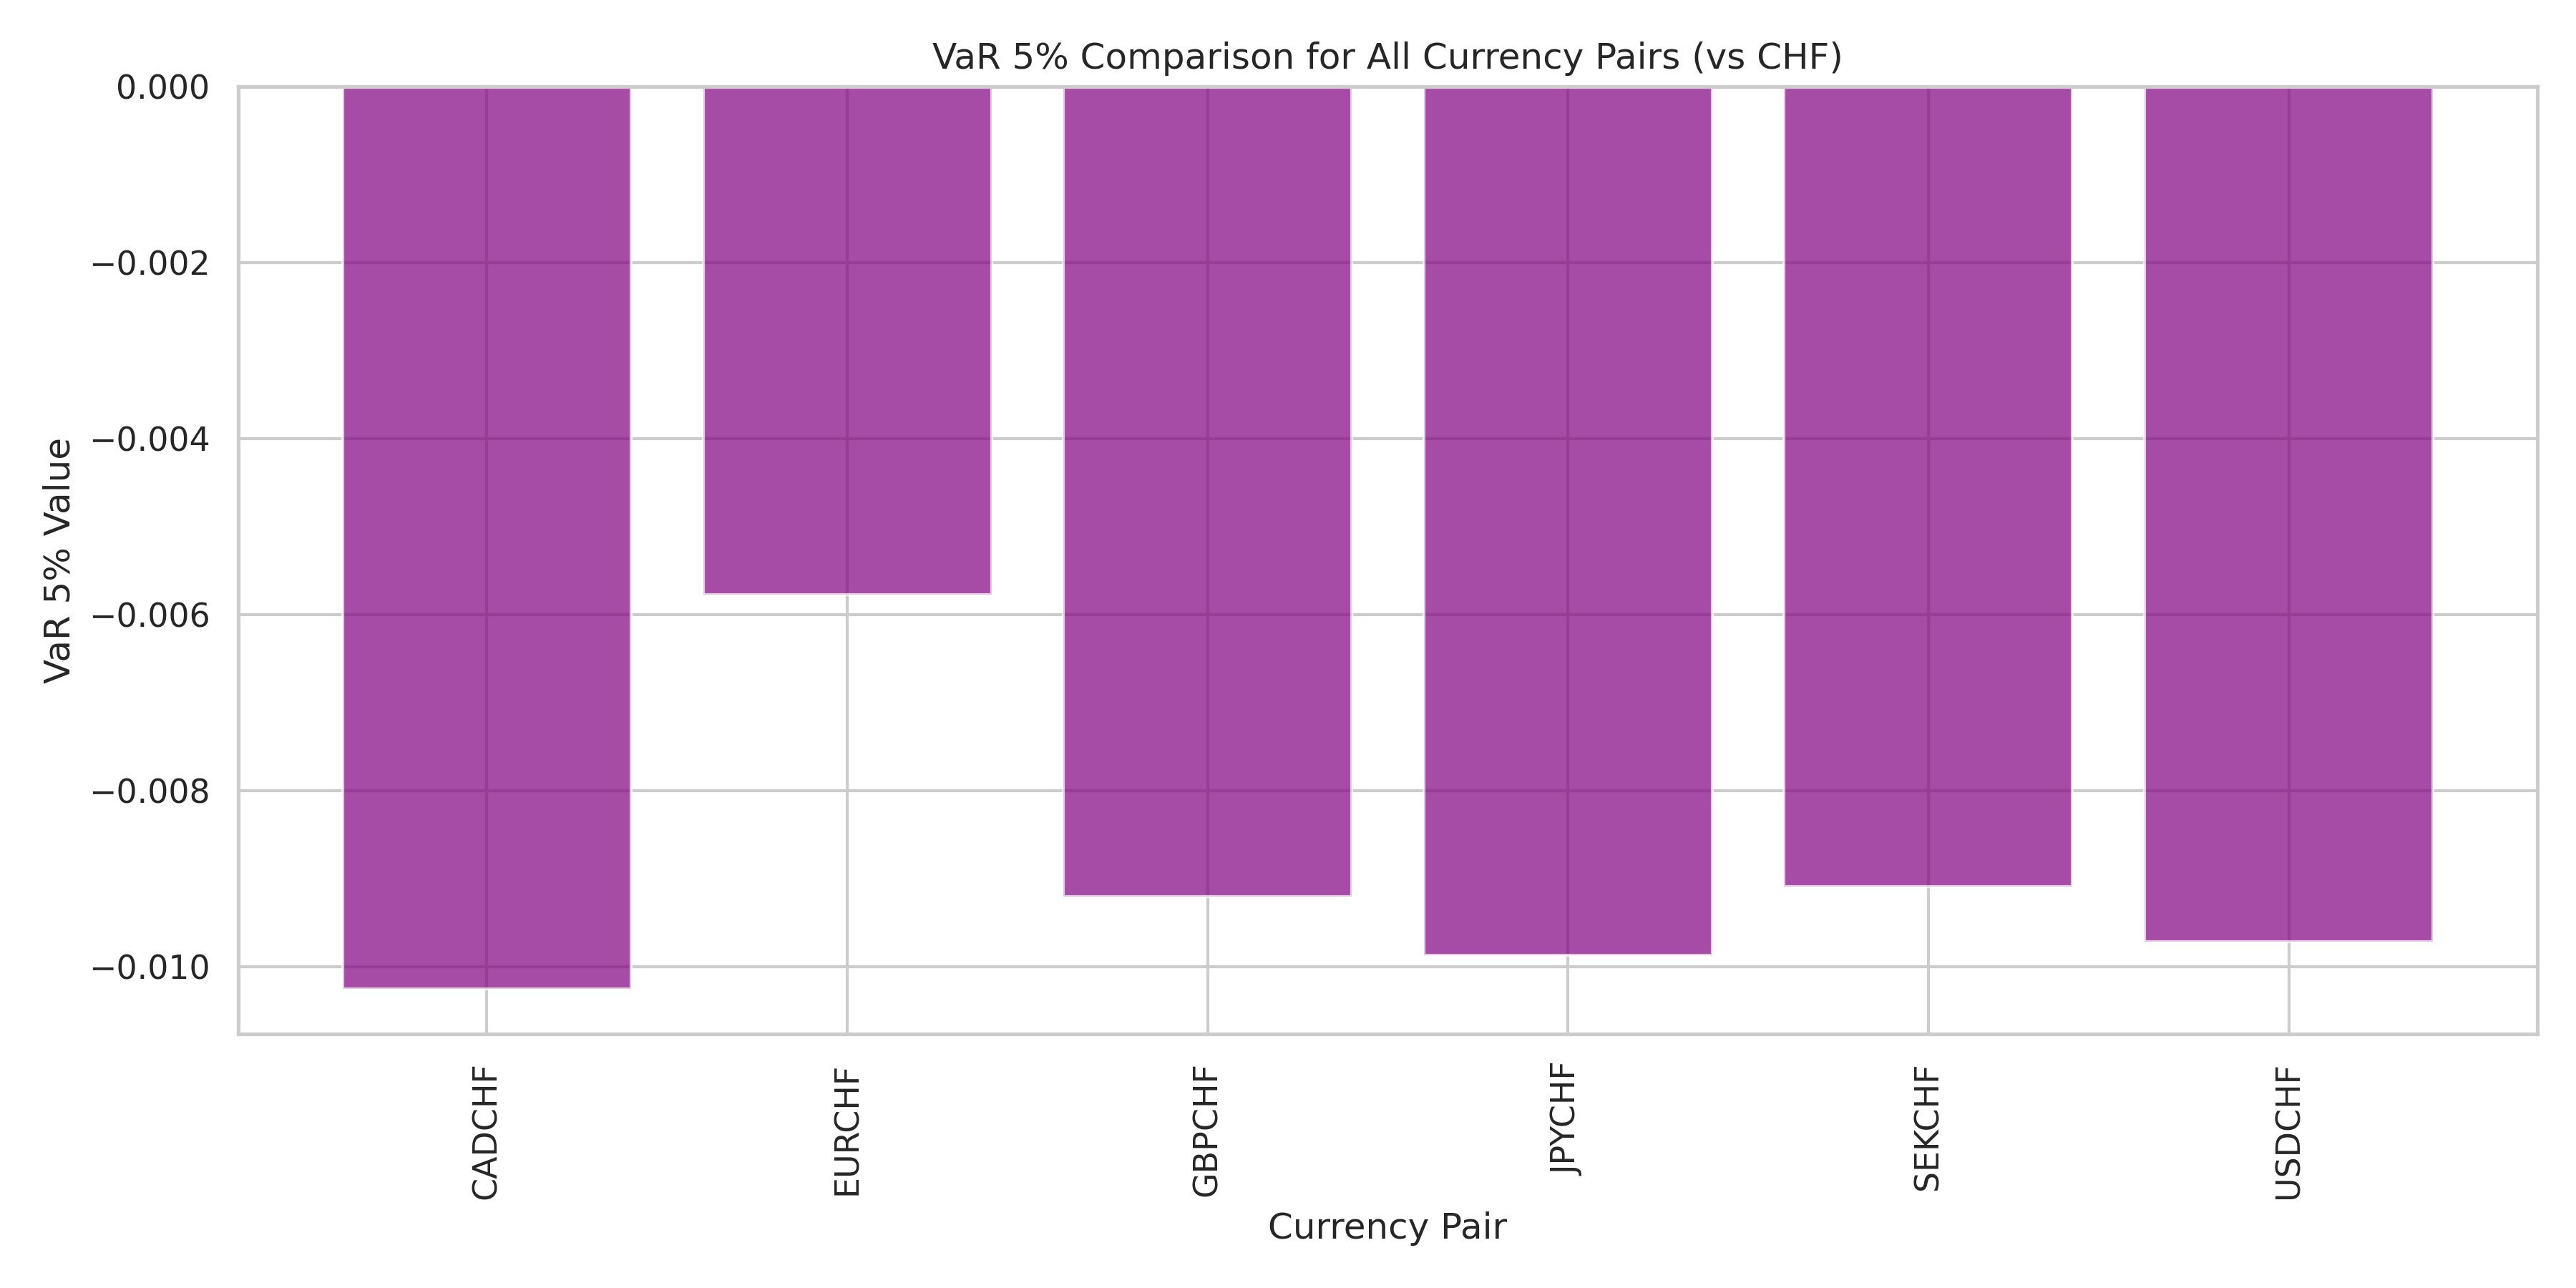
\includegraphics[width=0.48\linewidth]{reports/figures/var_5_percent_comparison_plot.png}
    \caption{Historical VaR of G10 currencies.}
    \label{fig:historical_VaR}
\end{figure}

\begin{table}[!ht]
    \centering
    \scalebox{0.48}{%
    \begin{tabular}{|c|c|c|}
    \hline
        Currency Pair & Historical VaR (5\%) & Monte Carlo VaR (5\%) \\ \hline
        AUDCHF & \textbf{-0.011509} & \textbf{-0.016160} \\ \hline
        CADCHF & -0.010249 & -0.009102 \\ \hline
        EURCHF & -0.005769 & -0.005250 \\ \hline
        GBPCHF & -0.009199 & -0.009942 \\ \hline
        JPYCHF & -0.009865 & -0.009910 \\ \hline
        NOKCHF & -0.010415 & -0.007992 \\ \hline
        NZDCHF & \textbf{-0.011832} & \textbf{-0.012486} \\ \hline
        SEKCHF & -0.009085 & \textbf{-0.011836} \\ \hline
        USDCHF & -0.009714 & -0.001894 \\ \hline
    \end{tabular}}
    \label{table:var}
    \caption{Historical VaR (5\%) and Monte Carlo VaR (5\%) for each currency pair.}
\end{table}
\end{frame}
% ---------------------------------------------------------------------------
\begin{frame}
\frametitle{Main Findings}
\framesubtitle{VaR Calculation}
However, in the Monte Carlo simulation, only AUD and NZD still indicated a VaR loss of over 1\%, suggesting that AUD and NZD exhibit high risk persistence as can be shown in Figures below.

\begin{figure}[h]
    \centering   
    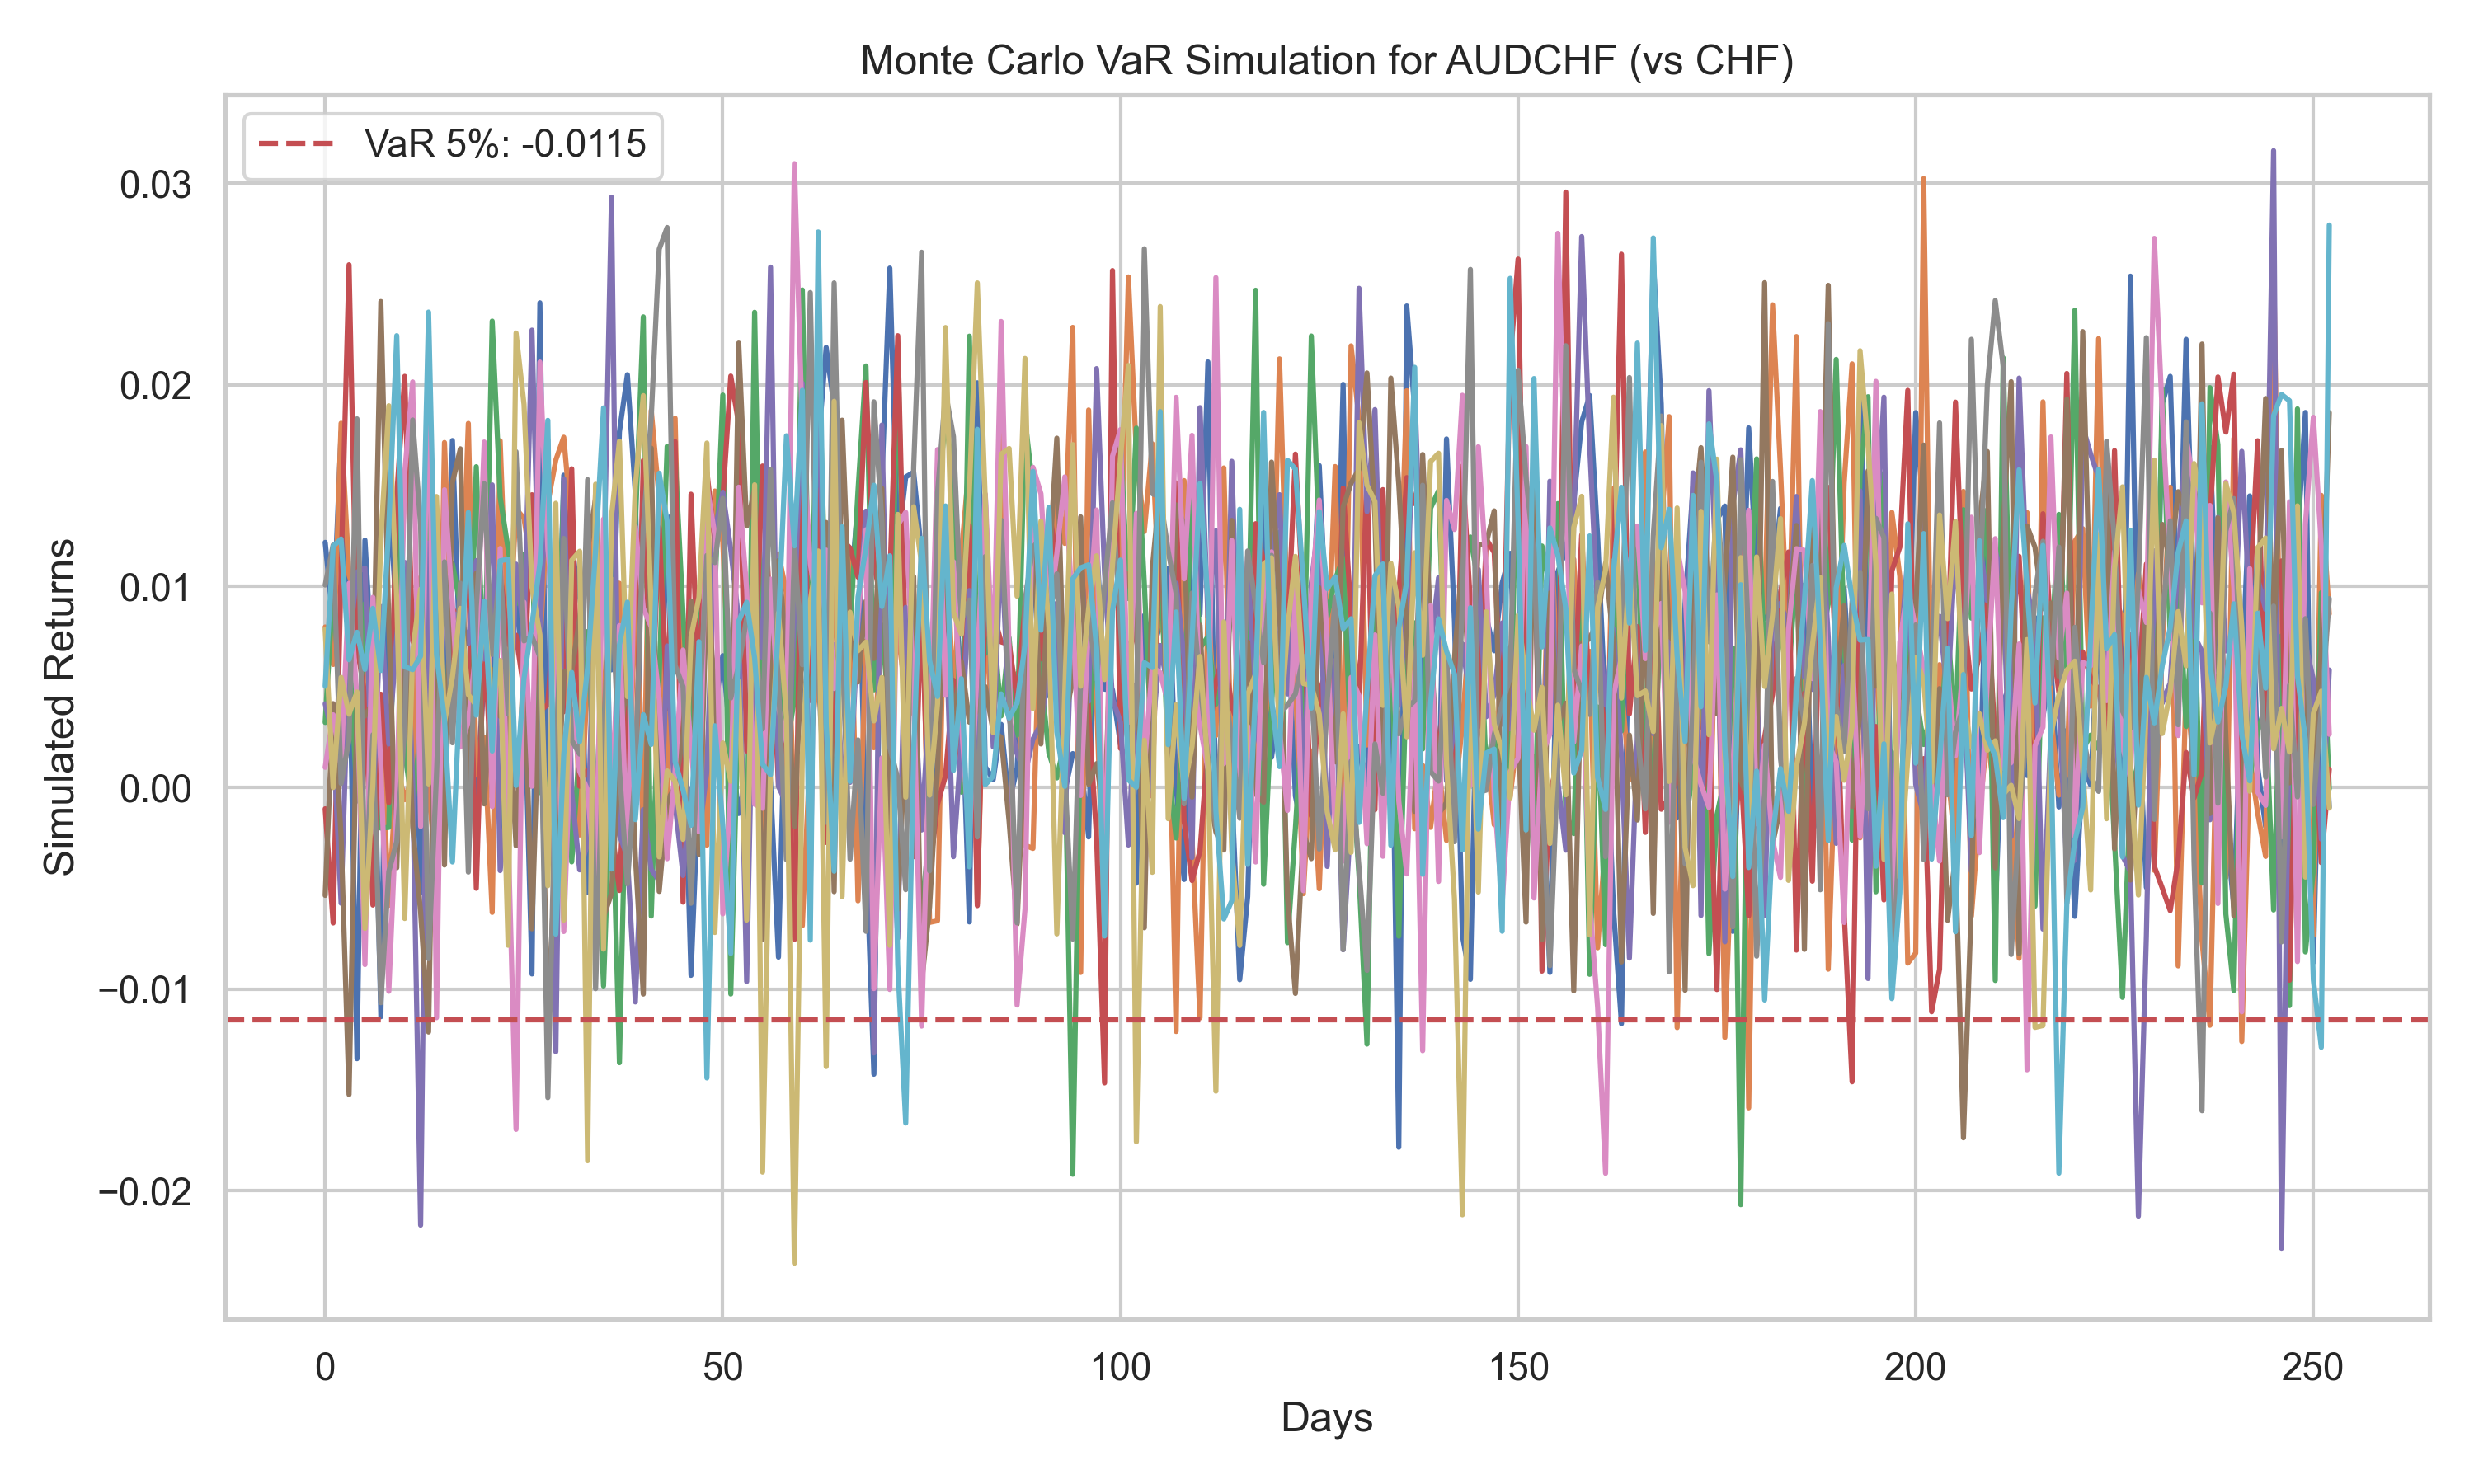
\includegraphics[width=0.48\linewidth]{reports/figures/monte_carlo_var_simulation_AUDCHF_vs_CHF.png}  \label{fig:monte_carlo_var_simulation_AUDCHF_vs_CHF}
    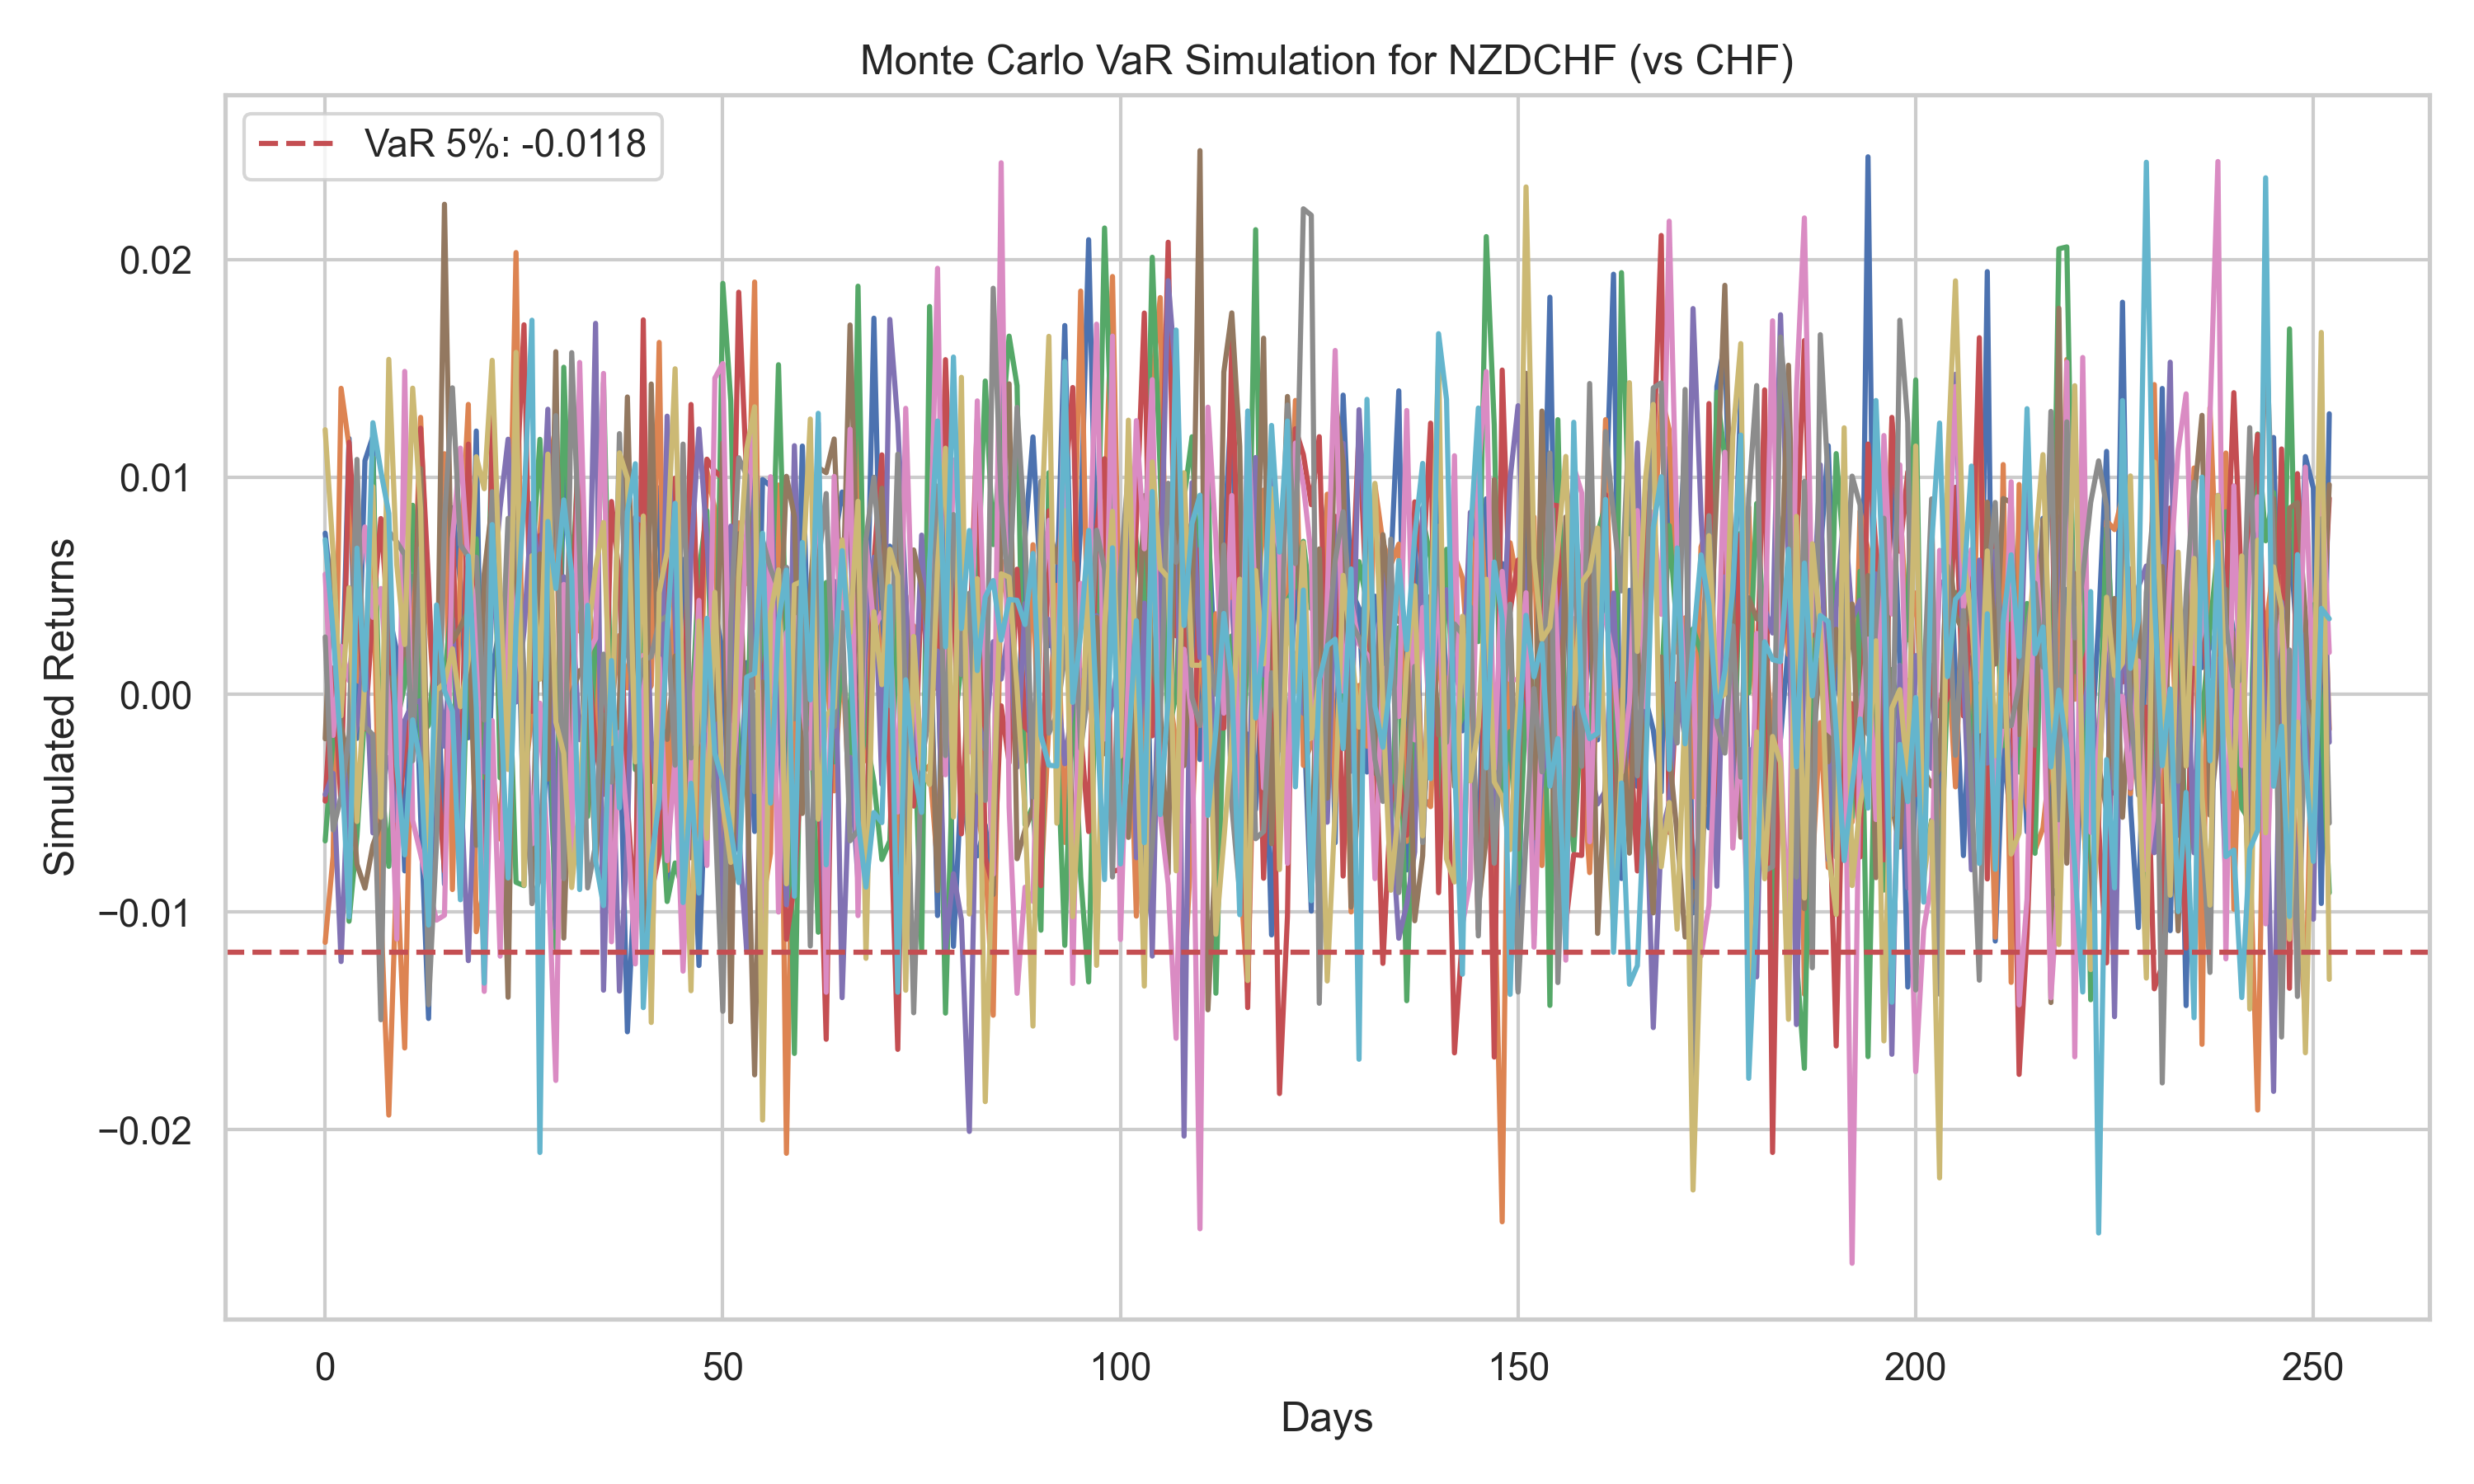
\includegraphics[width=0.48\linewidth]{reports/figures/monte_carlo_var_simulation_NZDCHF_vs_CHF.png}   \label{fig:monte_carlo_var_simulation_NZDCHF_vs_CHF}
    \caption{\footnotesize Monte Carlo VaR Simulation of AUDCHF vs. CHF (left) and NZDCHF vs. CHF (right)}  
\end{figure}
\end{frame}
% ---------------------------------------------------------------------------
\begin{frame}
\frametitle{Main Findings}
\framesubtitle{VaR Calculation}
\begin{itemize}
    \item Both historical data and simulations indicate that these two currencies carry sustained risk characteristics, and investors should be particularly cautious when considering these currency pairs.
    \item SEK shows increased risk in
    the Monte Carlo simulation, with its VaR exceeding 1\%, transitioning from a low-risk to a high-risk profile. This suggests that SEK may face greater uncertainty and potential risks in future market volatility.
\end{itemize}
\end{frame}
% ---------------------------------------------------------------------------
\begin{frame}
\frametitle{Main Findings}
\framesubtitle{Price Simulation}
GBP shows the most significant price volatility, approximately 0.4, indicating high future price uncertainty for GBP pairs. Volatility of AUDCHF is around 0.33, and of NZDCHF is approximately
0.27, also reflecting considerable price uncertainty.
\begin{figure}[h]
    \centering  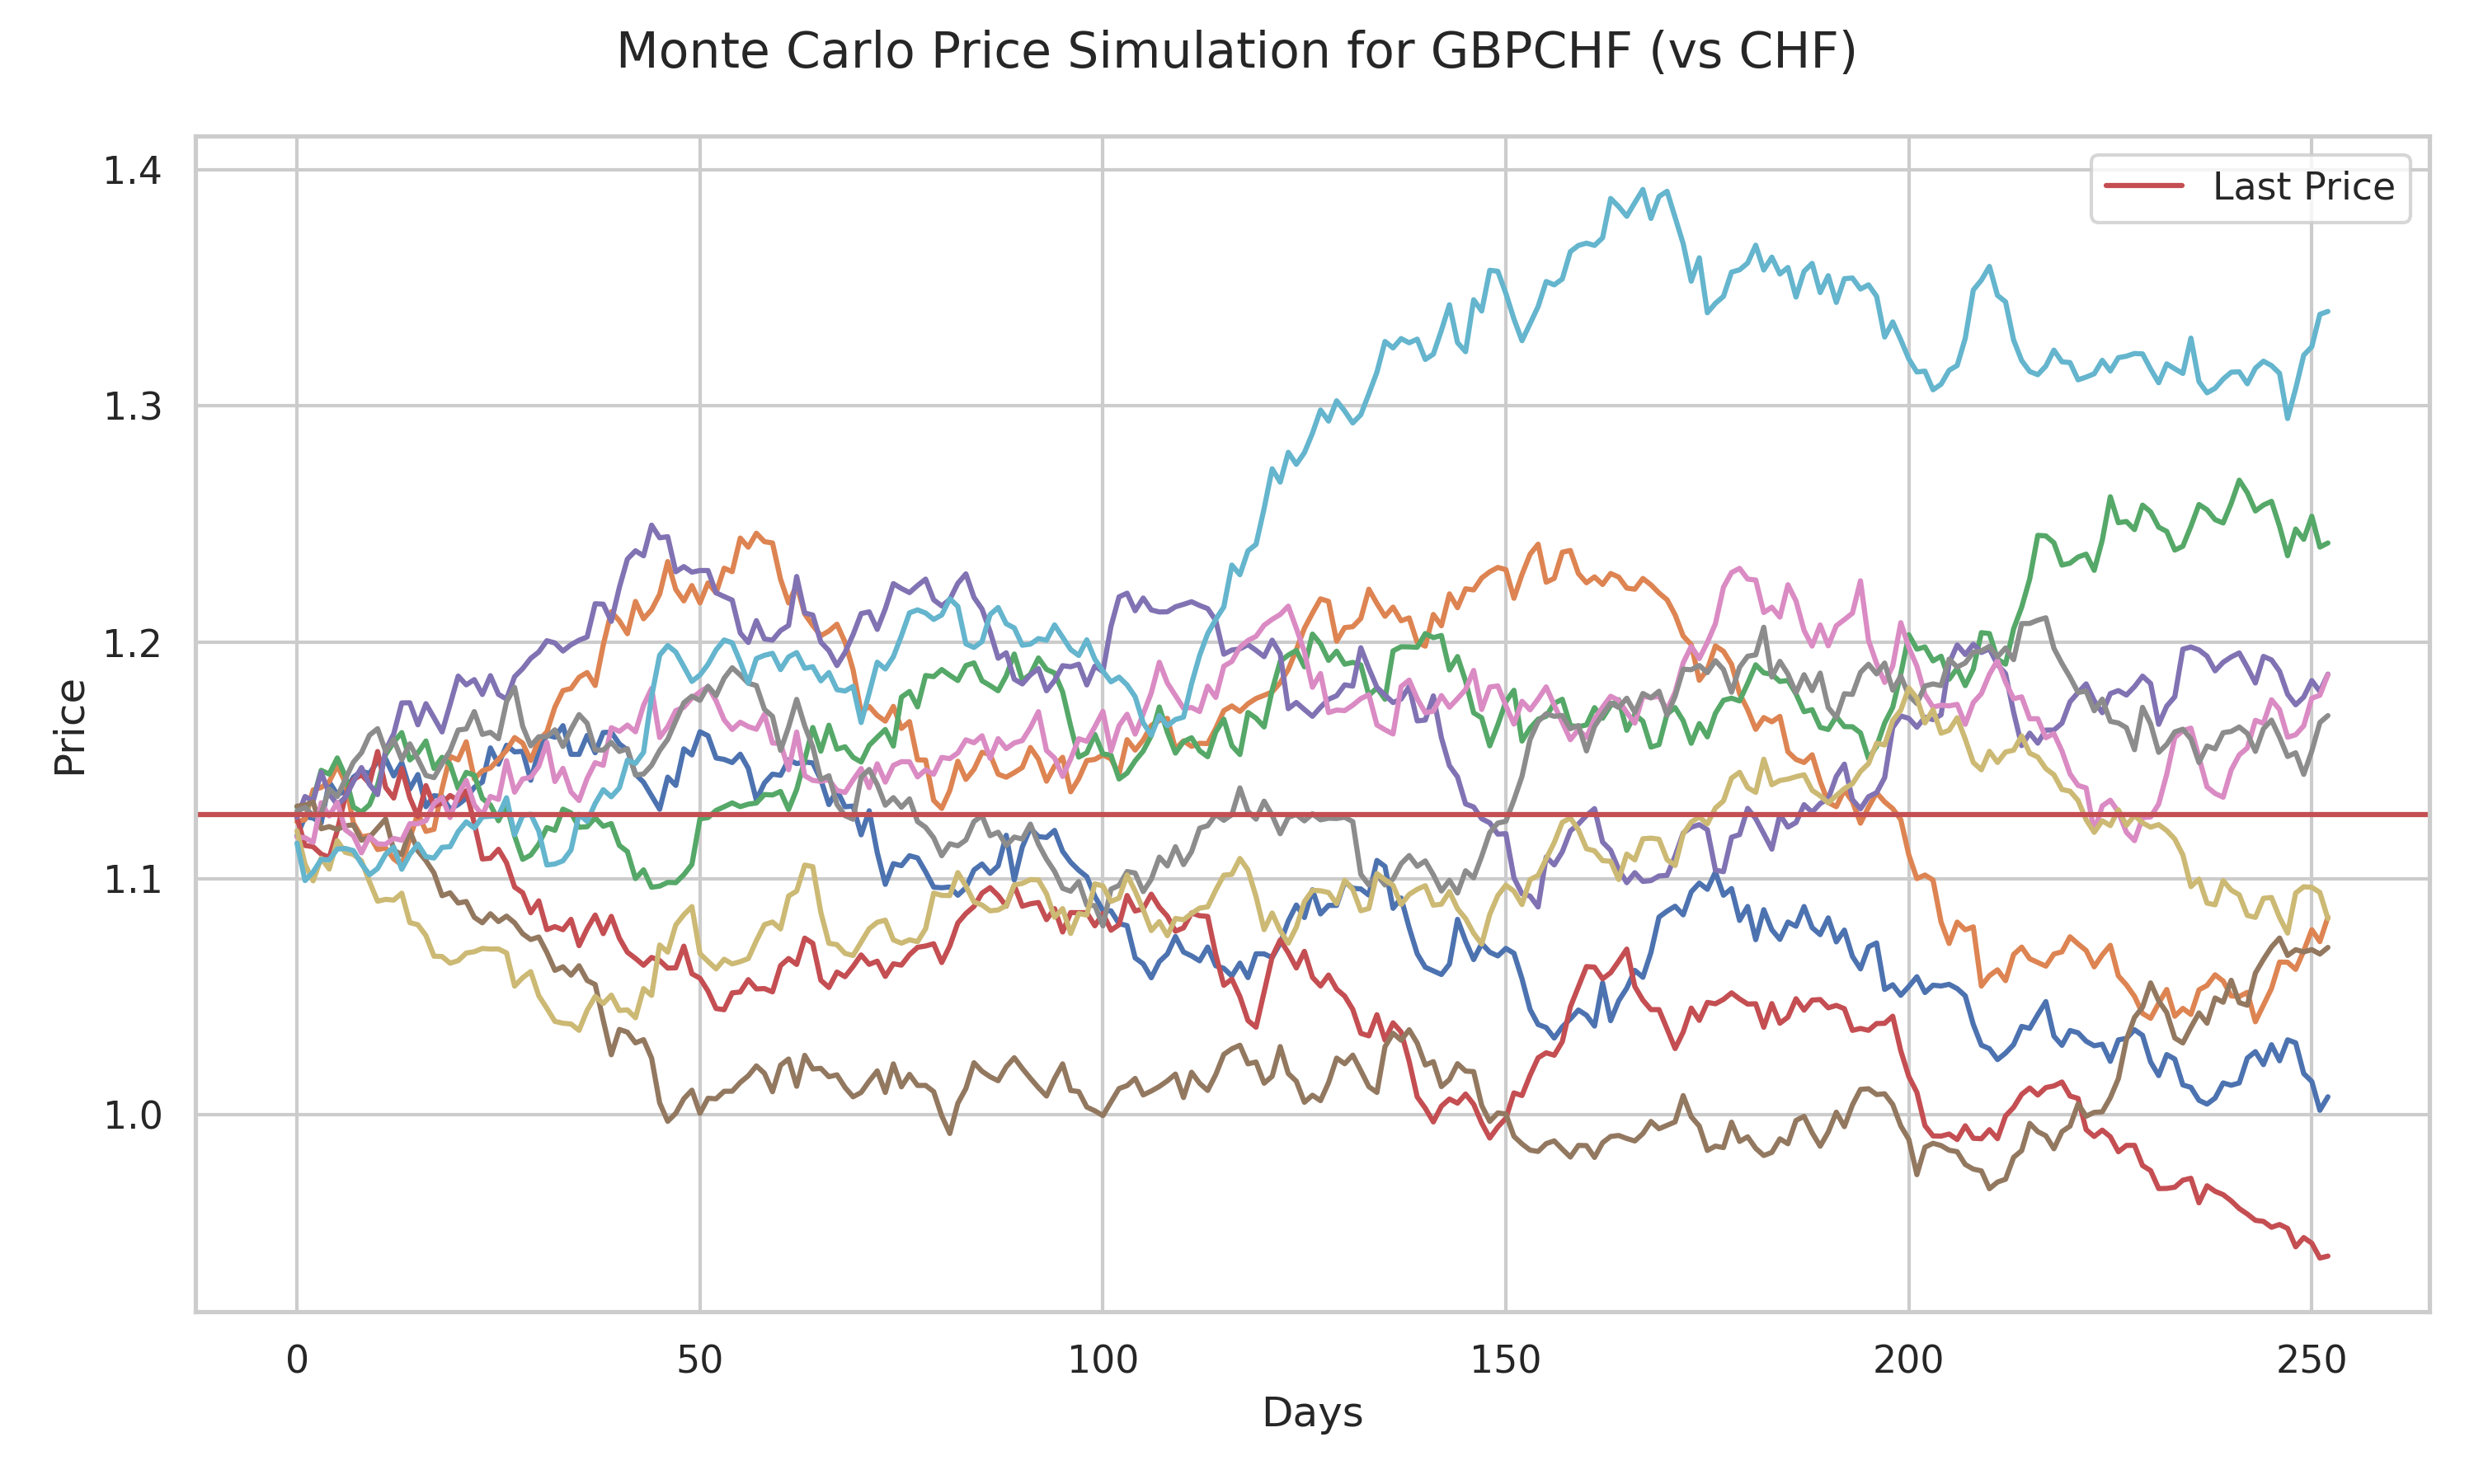
\includegraphics[width=0.75\linewidth]{reports/figures/monte_carlo_price_simulation_GBPCHF_vs_CHF.png}
    \caption{Monte Carlo Price Simulation of GBPCHF vs. CHF}  \label{fig:monte_carlo_price_simulation_GBPCHF_vs_CHF}
\end{figure}
\end{frame}
% ---------------------------------------------------------------------------
\begin{frame}
\frametitle{Main Findings}
\framesubtitle{Price Simulation}
\begin{figure}
    \centering   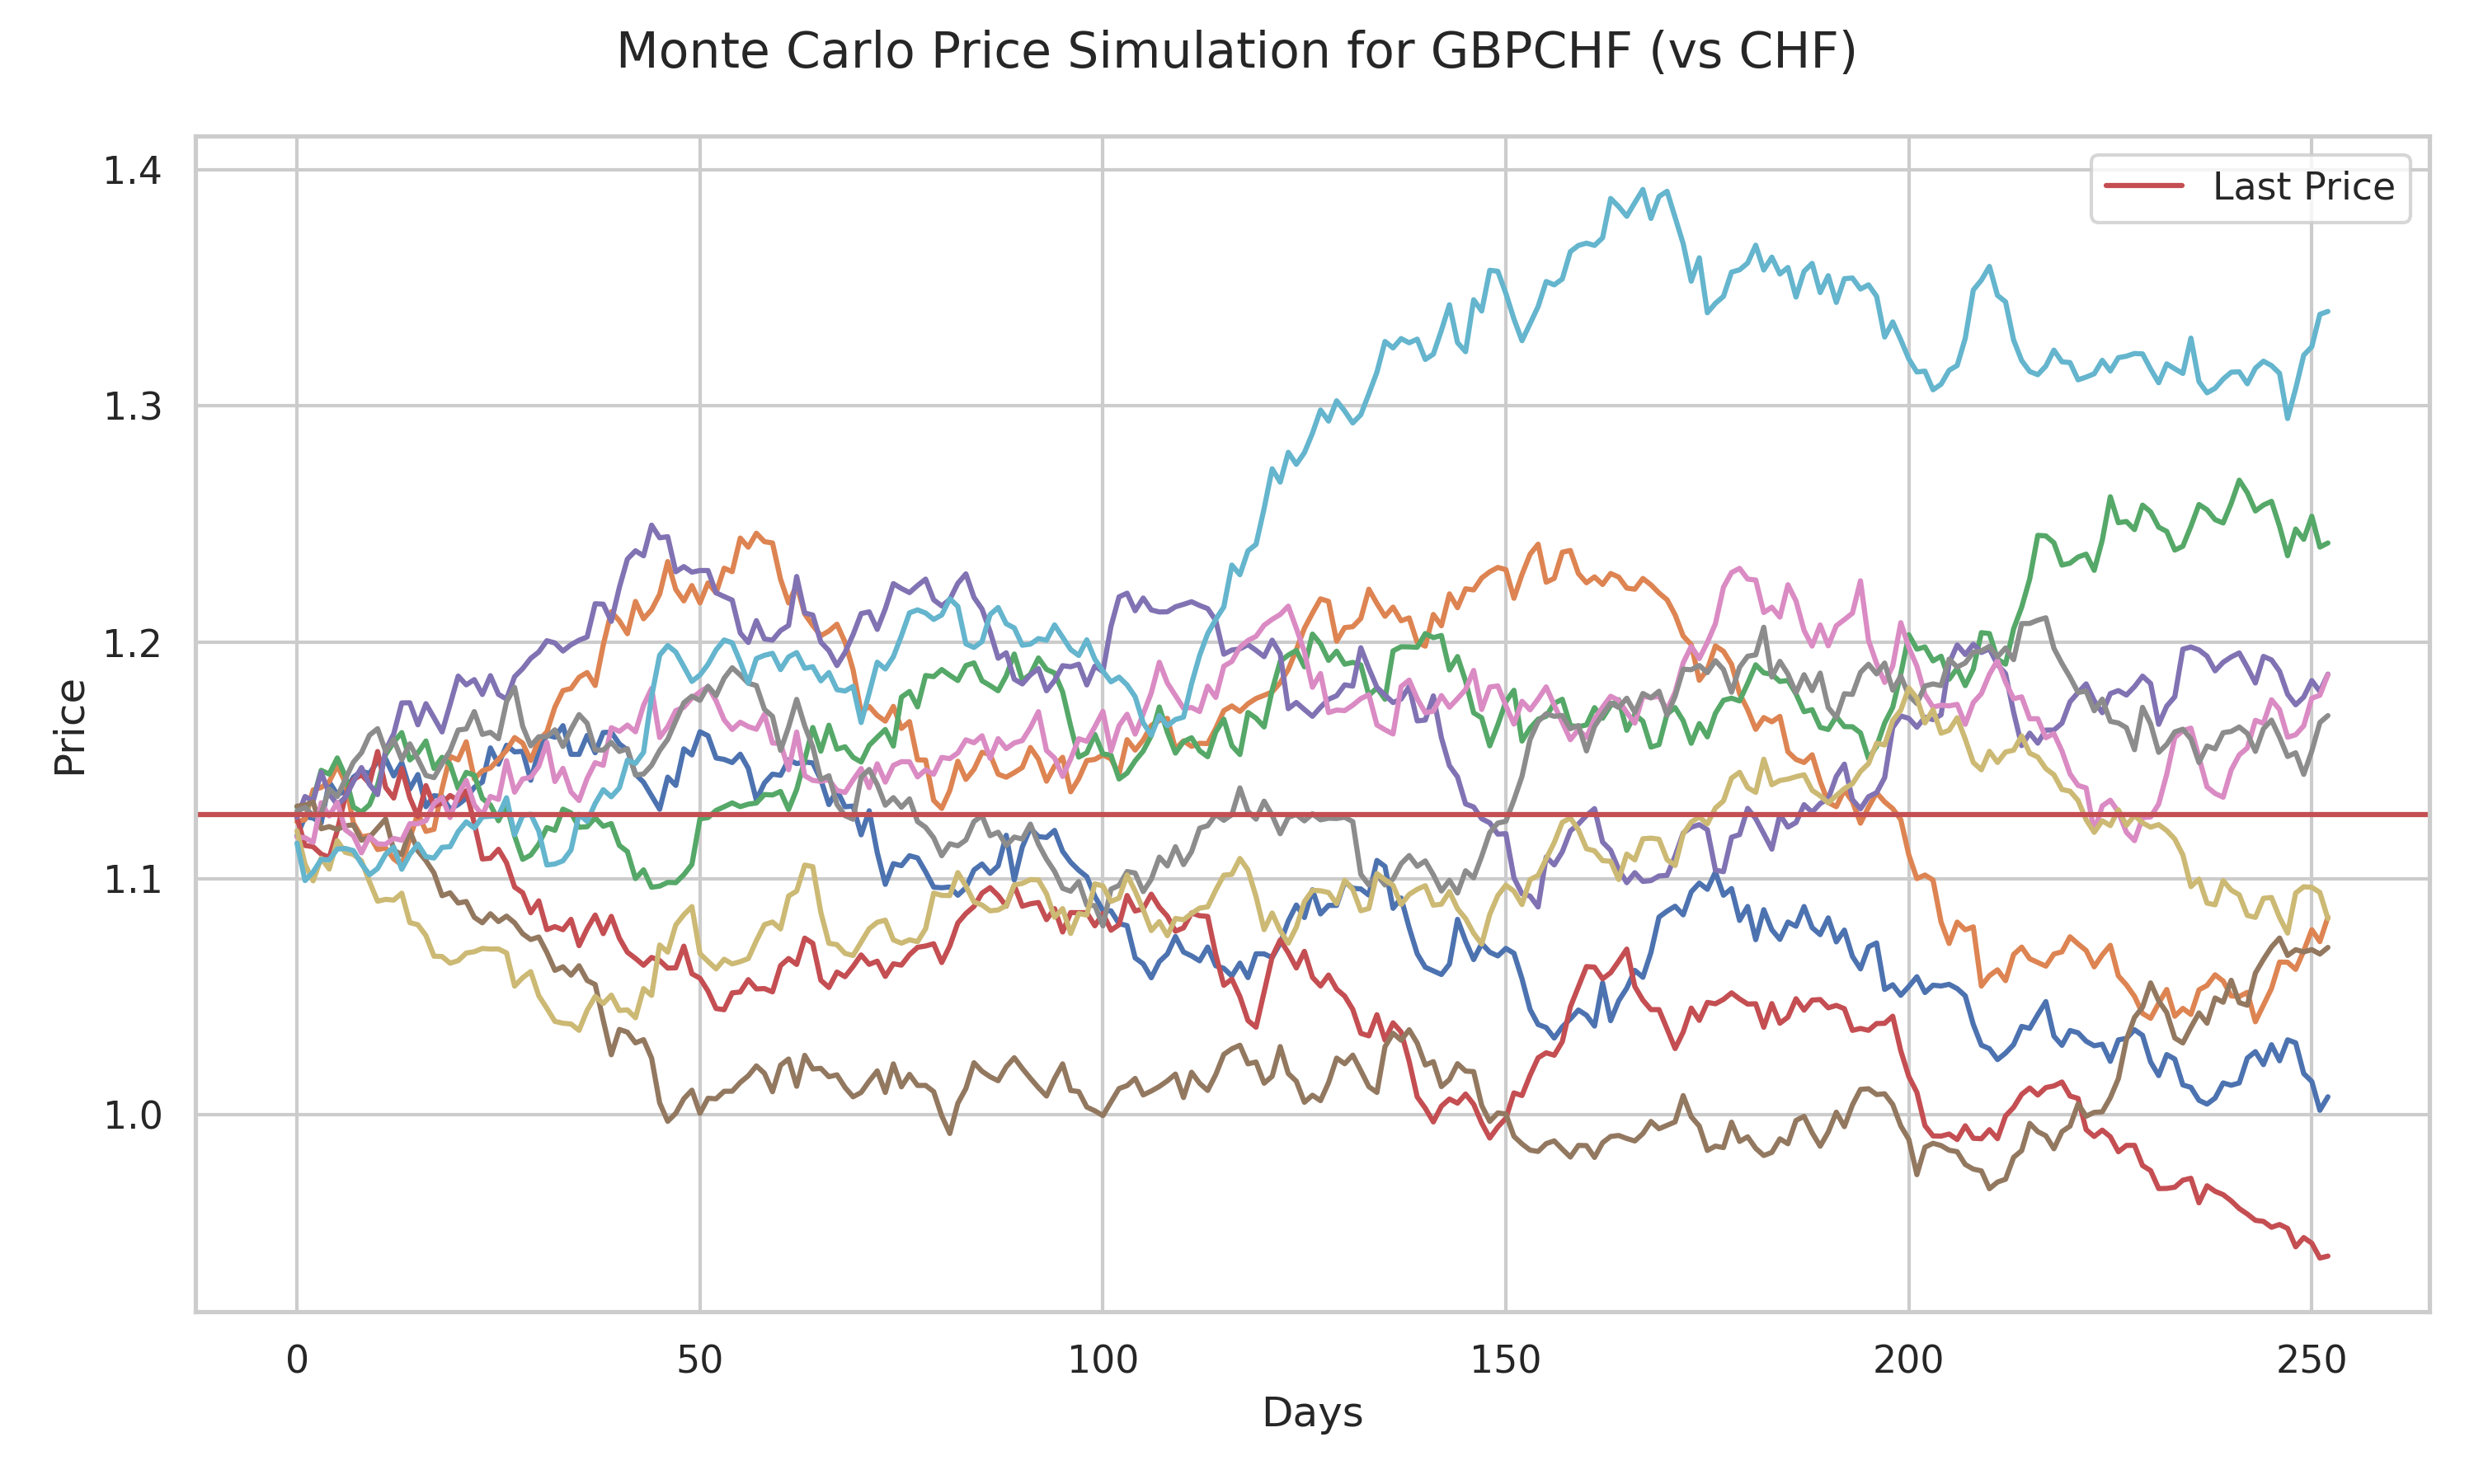
\includegraphics[width=0.48\linewidth]{reports/figures/monte_carlo_price_simulation_GBPCHF_vs_CHF.png} \label{fig:monte_carlo_price_simulation_GBPCHF_vs_CHF}
    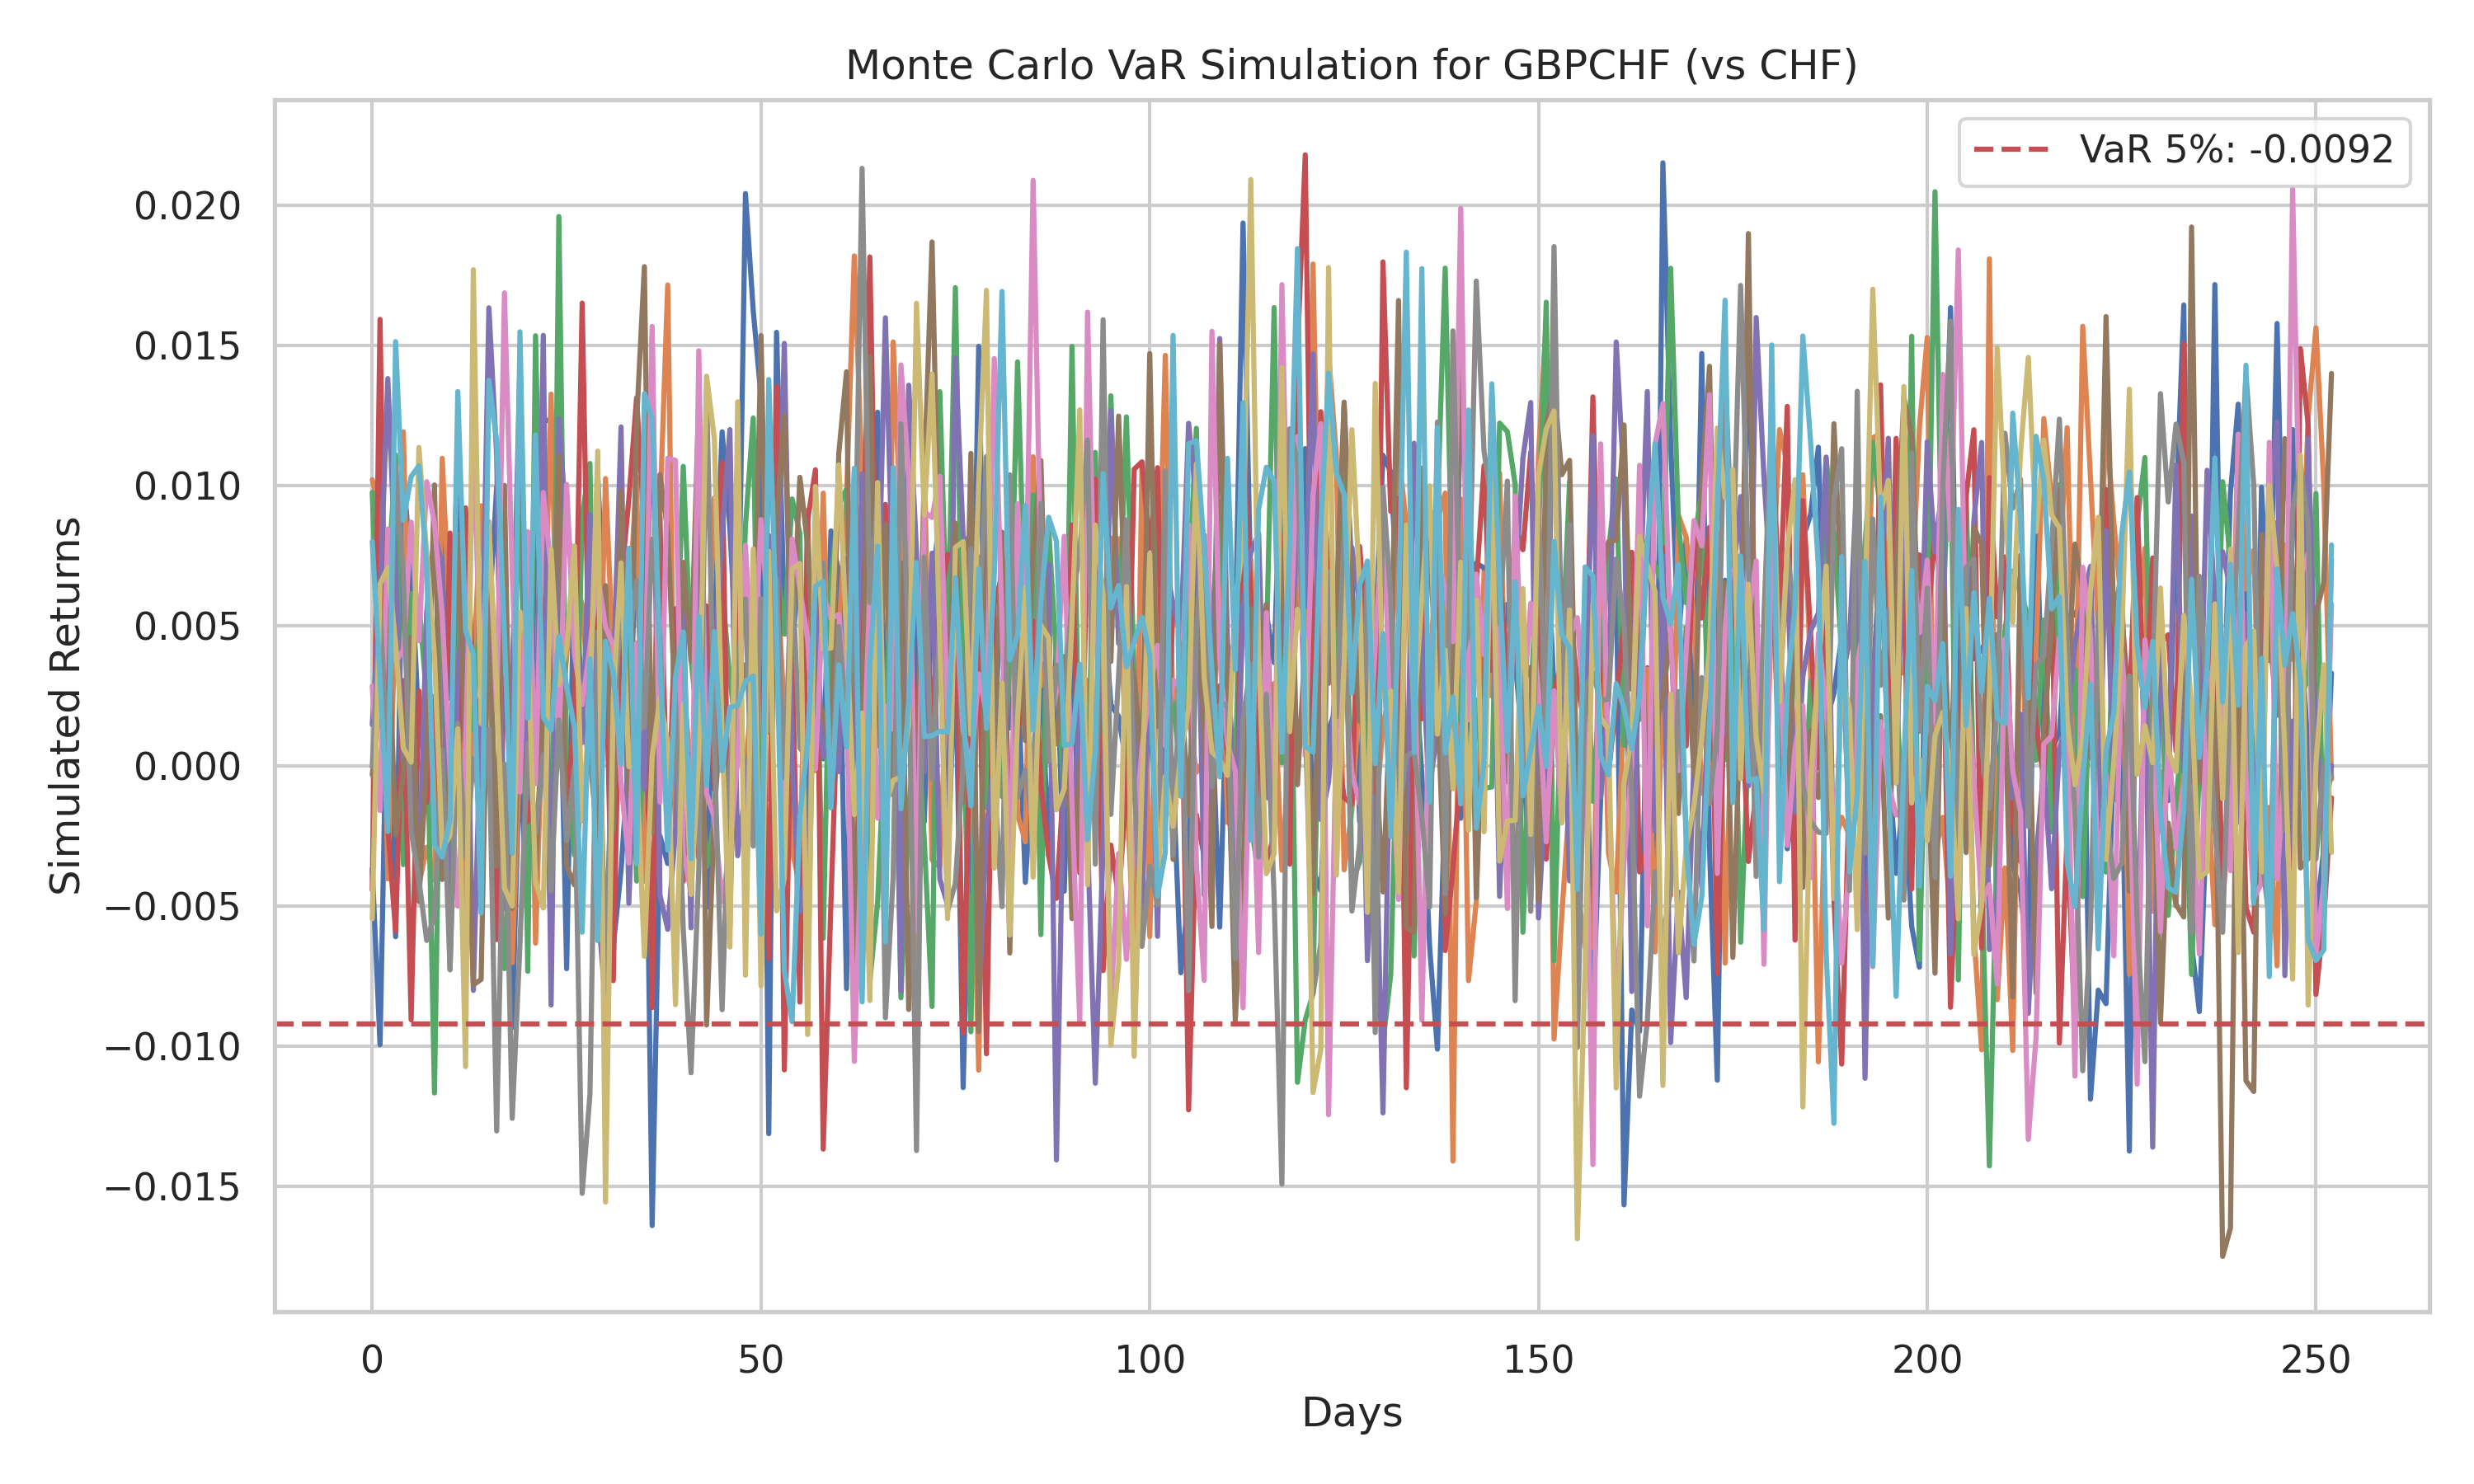
\includegraphics[width=0.48\linewidth]{reports/figures/monte_carlo_var_simulation_GBPCHF_vs_CHF.png} \label{fig:monte_carlo_var_simulation_GBPCHF_vs_CHF}
    \caption{\footnotesize Monte Carlo price siulation (left) and VaR simulation (right) for GBP-CHF.}
\end{figure}
\end{frame}
% ---------------------------------------------------------------------------
\begin{frame}
\frametitle{Main Findings}
\framesubtitle{Regression Analysis}
\begin{figure}
    \centering  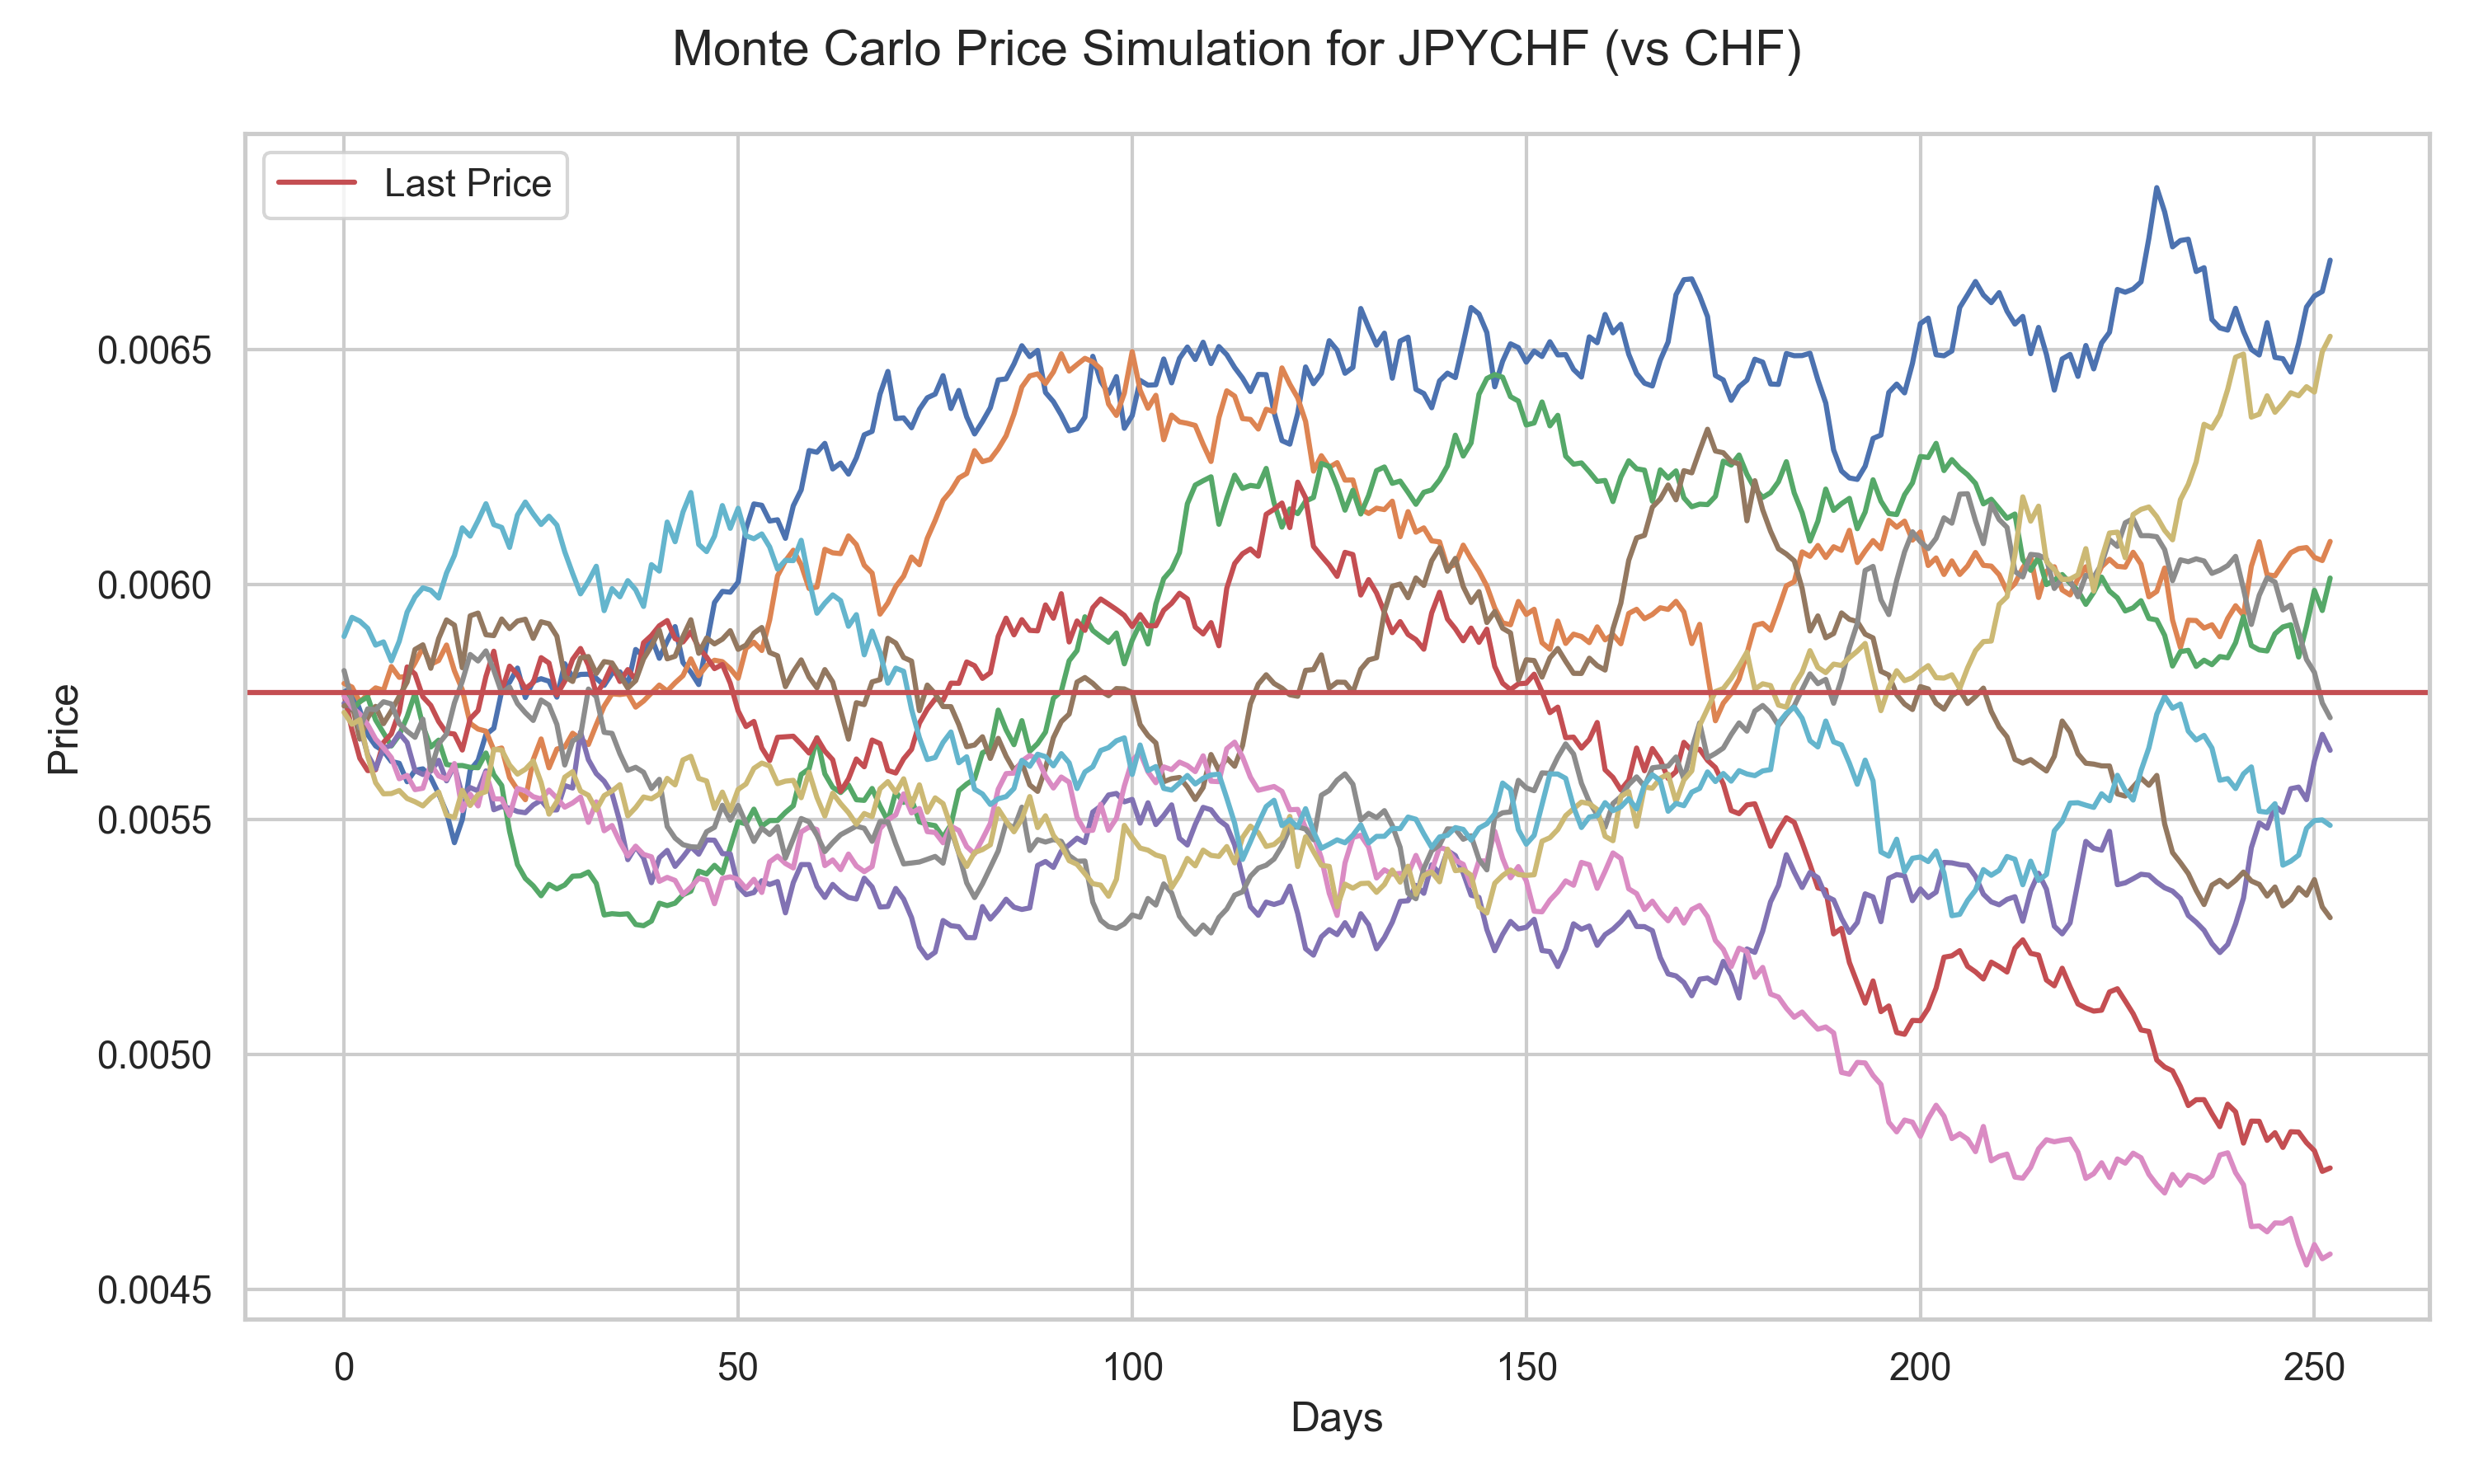
\includegraphics[width=0.48\linewidth]{reports/figures/monte_carlo_price_simulation_JPYCHF_vs_CHF.png}  \label{fig:monte_carlo_price_simulation_JPYCHF_vs_CHF}
    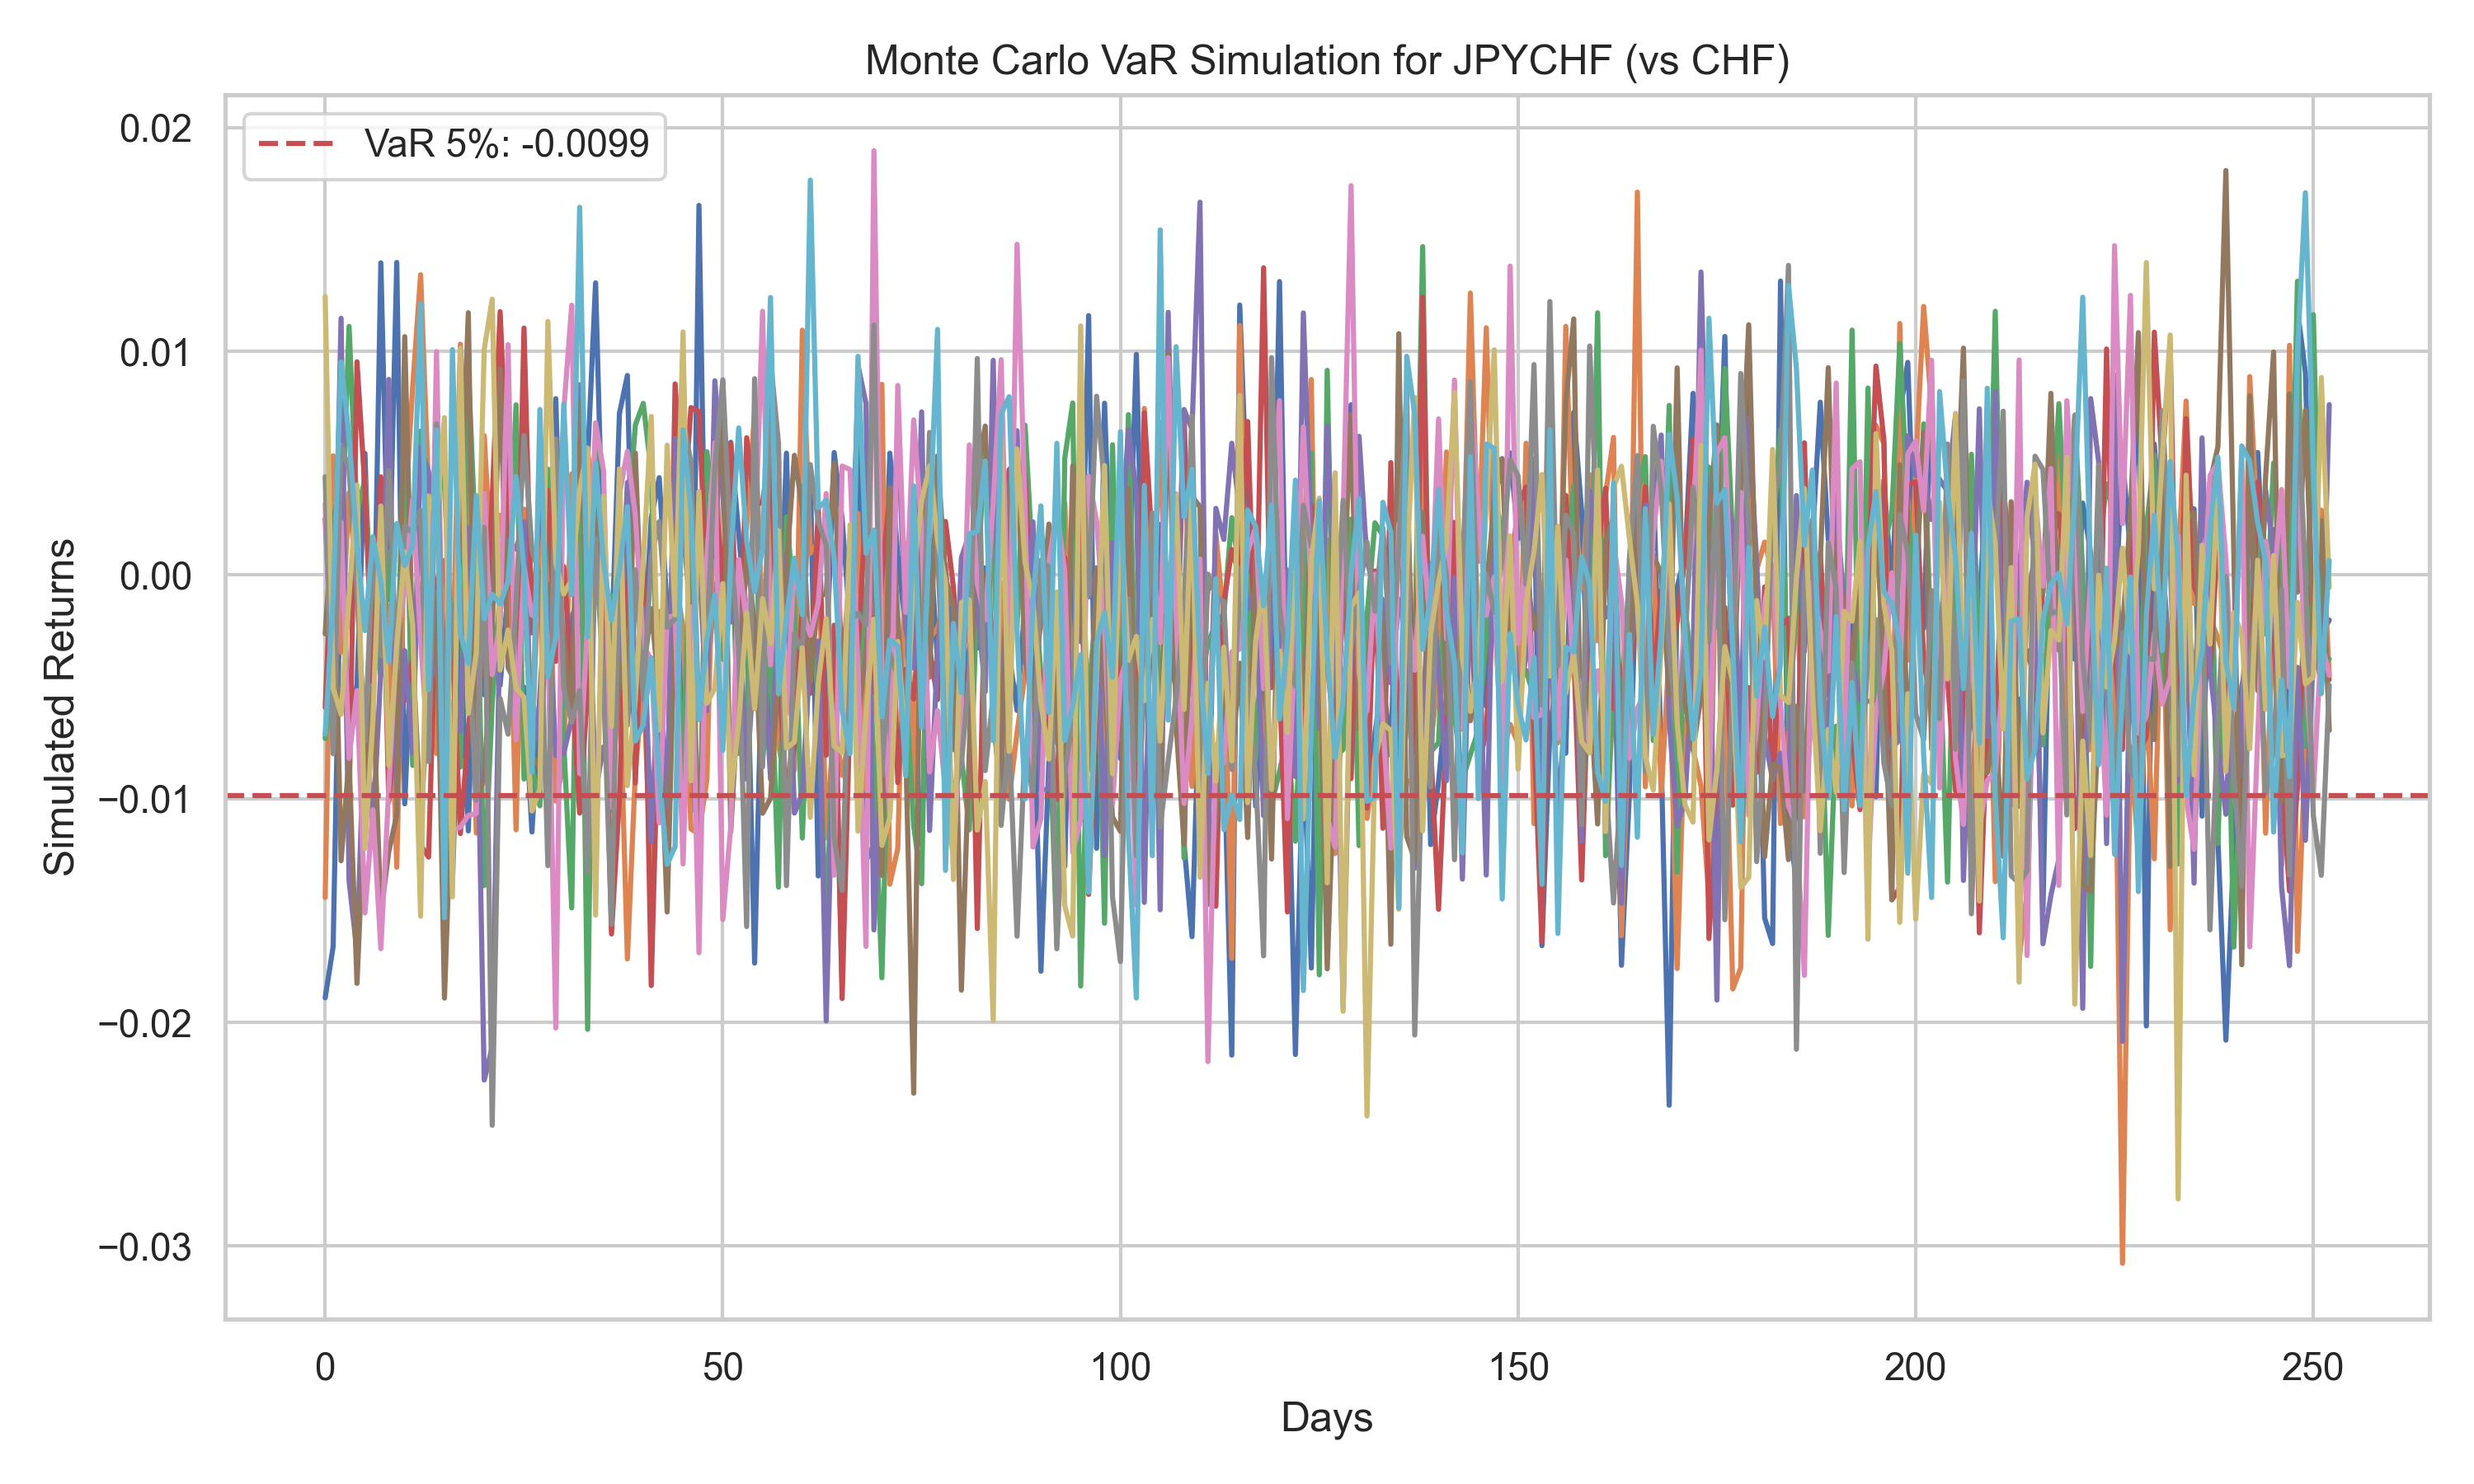
\includegraphics[width=0.48\linewidth]{reports/figures/monte_carlo_var_simulation_JPYCHF_vs_CHF.png}  \label{fig:monte_carlo_var_simulation_JPYCHF_vs_CHF}
    \caption{\footnotesize Monte Carlo price siulation (left) and VaR simulation (right) for JPY-CHF.}
\end{figure}
\begin{figure}
    \centering   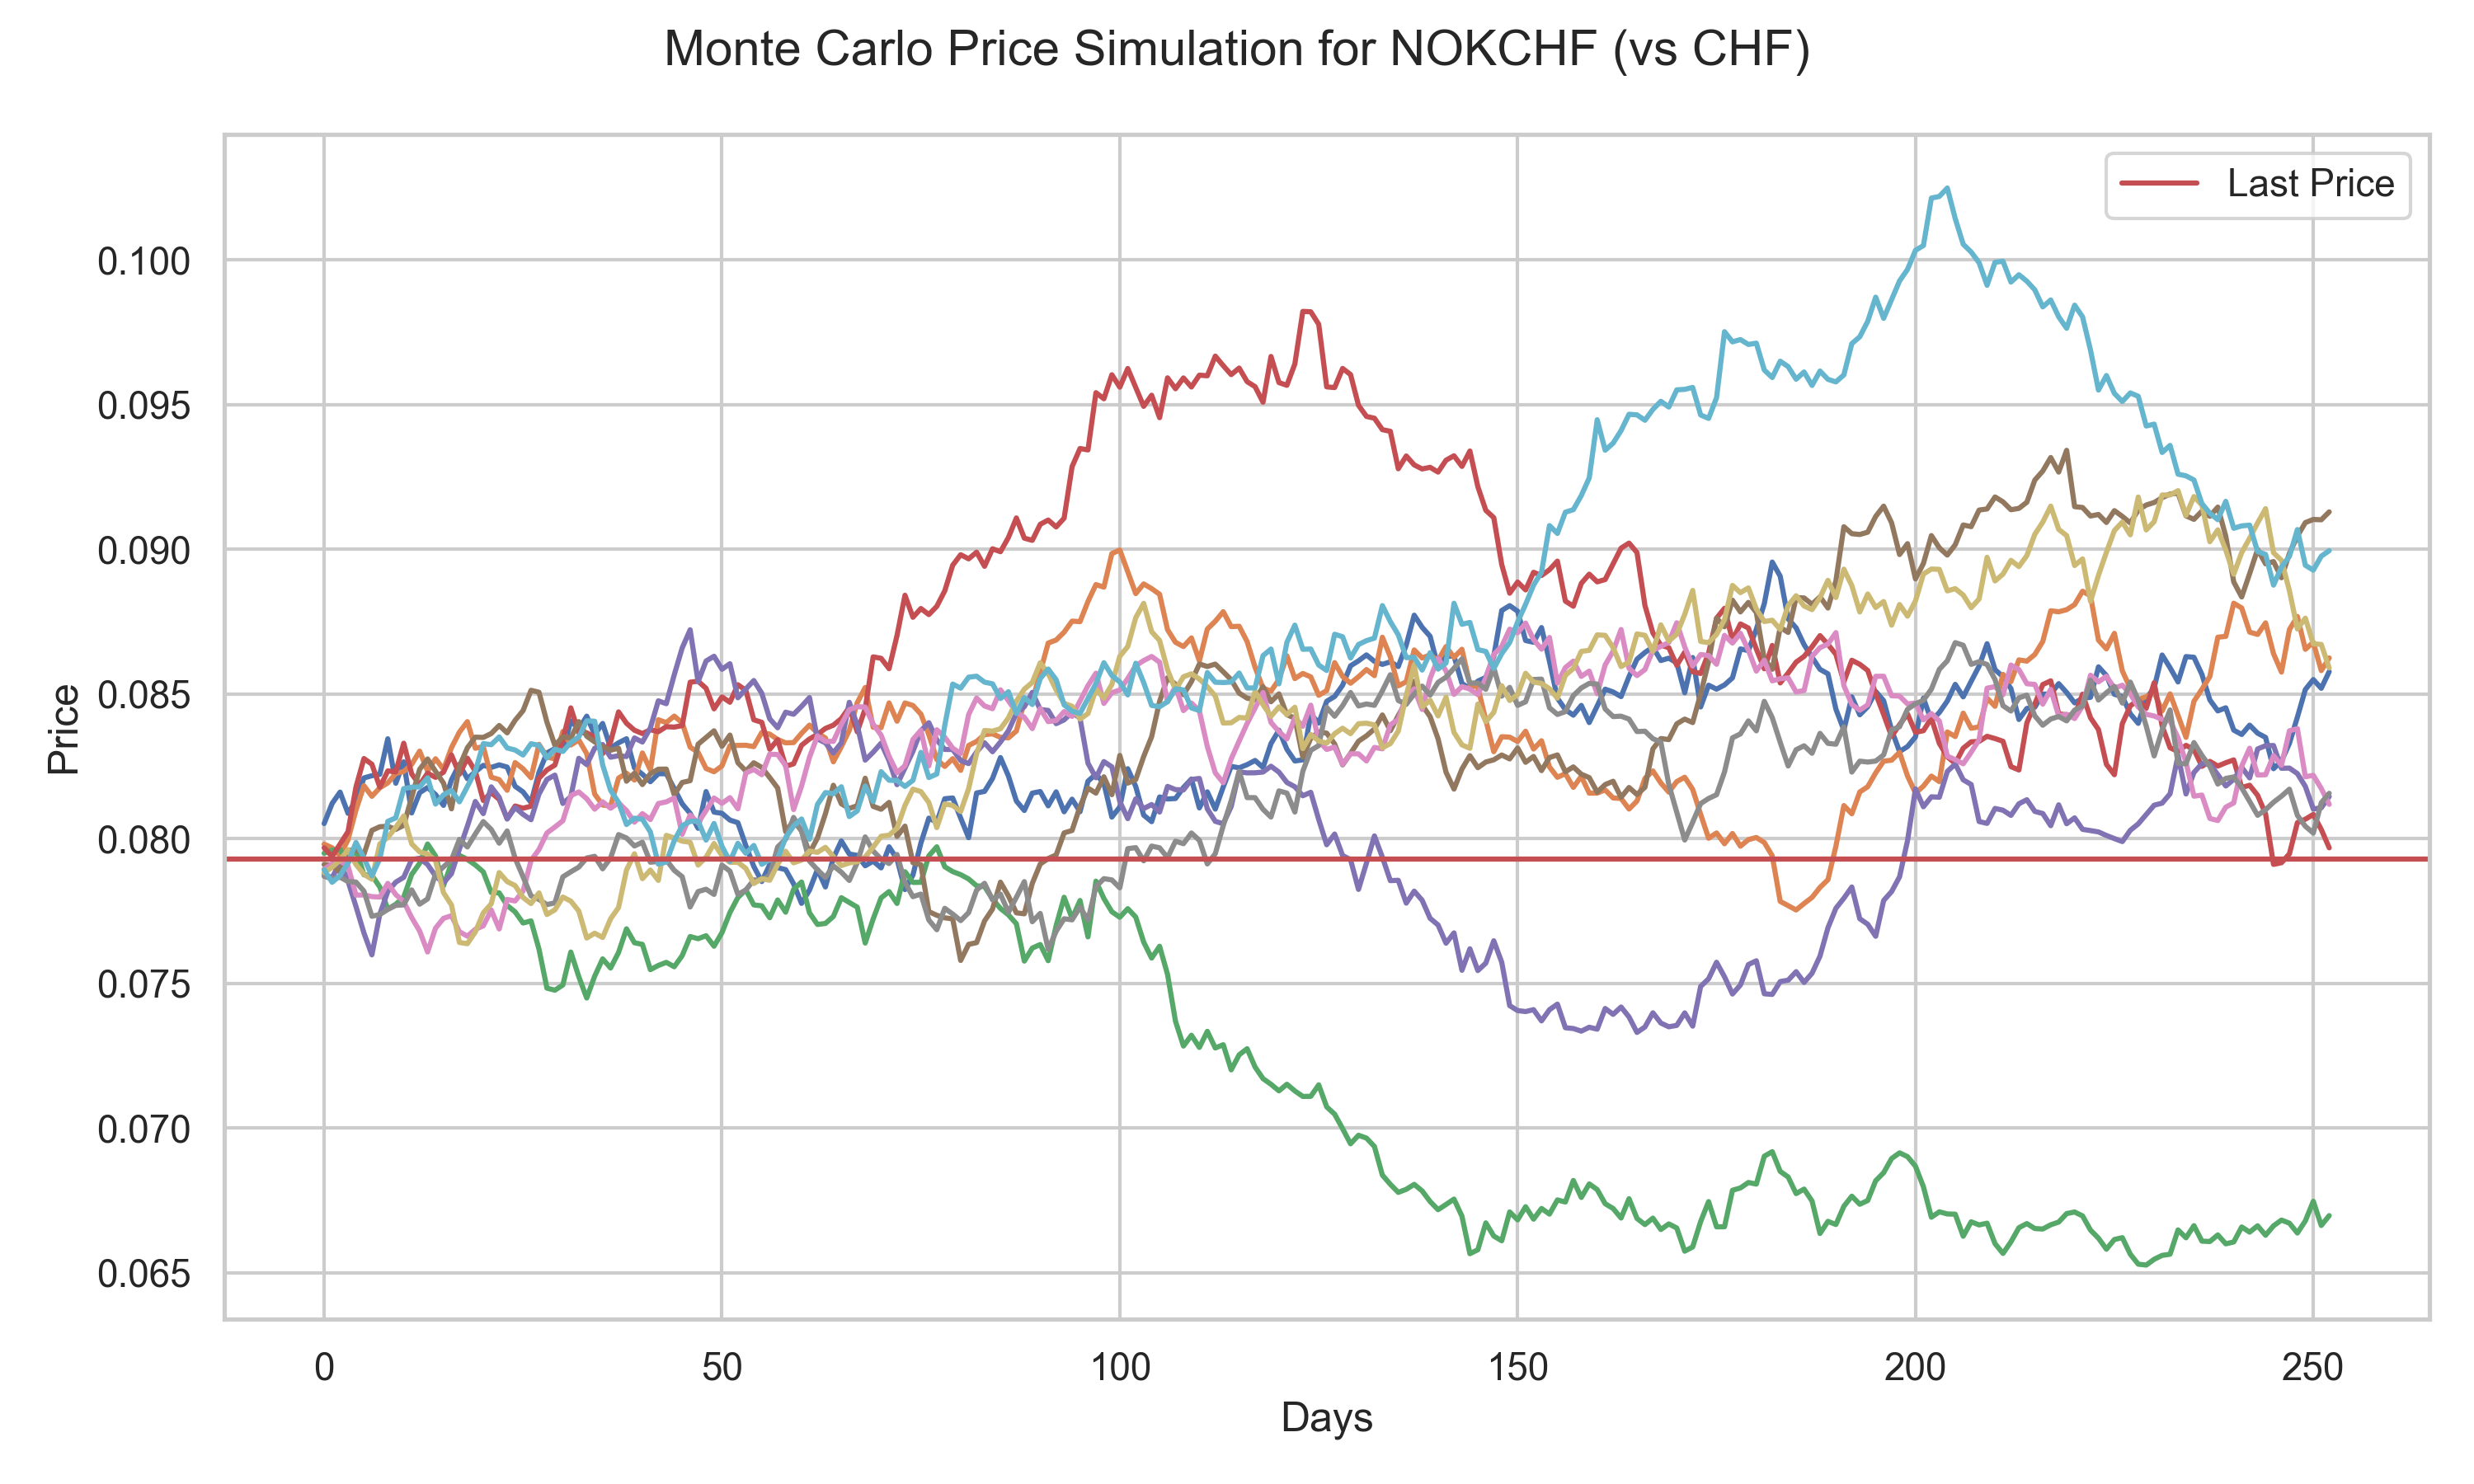
\includegraphics[width=0.48\linewidth]{reports/figures/monte_carlo_price_simulation_NOKCHF_vs_CHF.png} \label{fig:monte_carlo_price_simulation_NOKCHF_vs_CHF}
    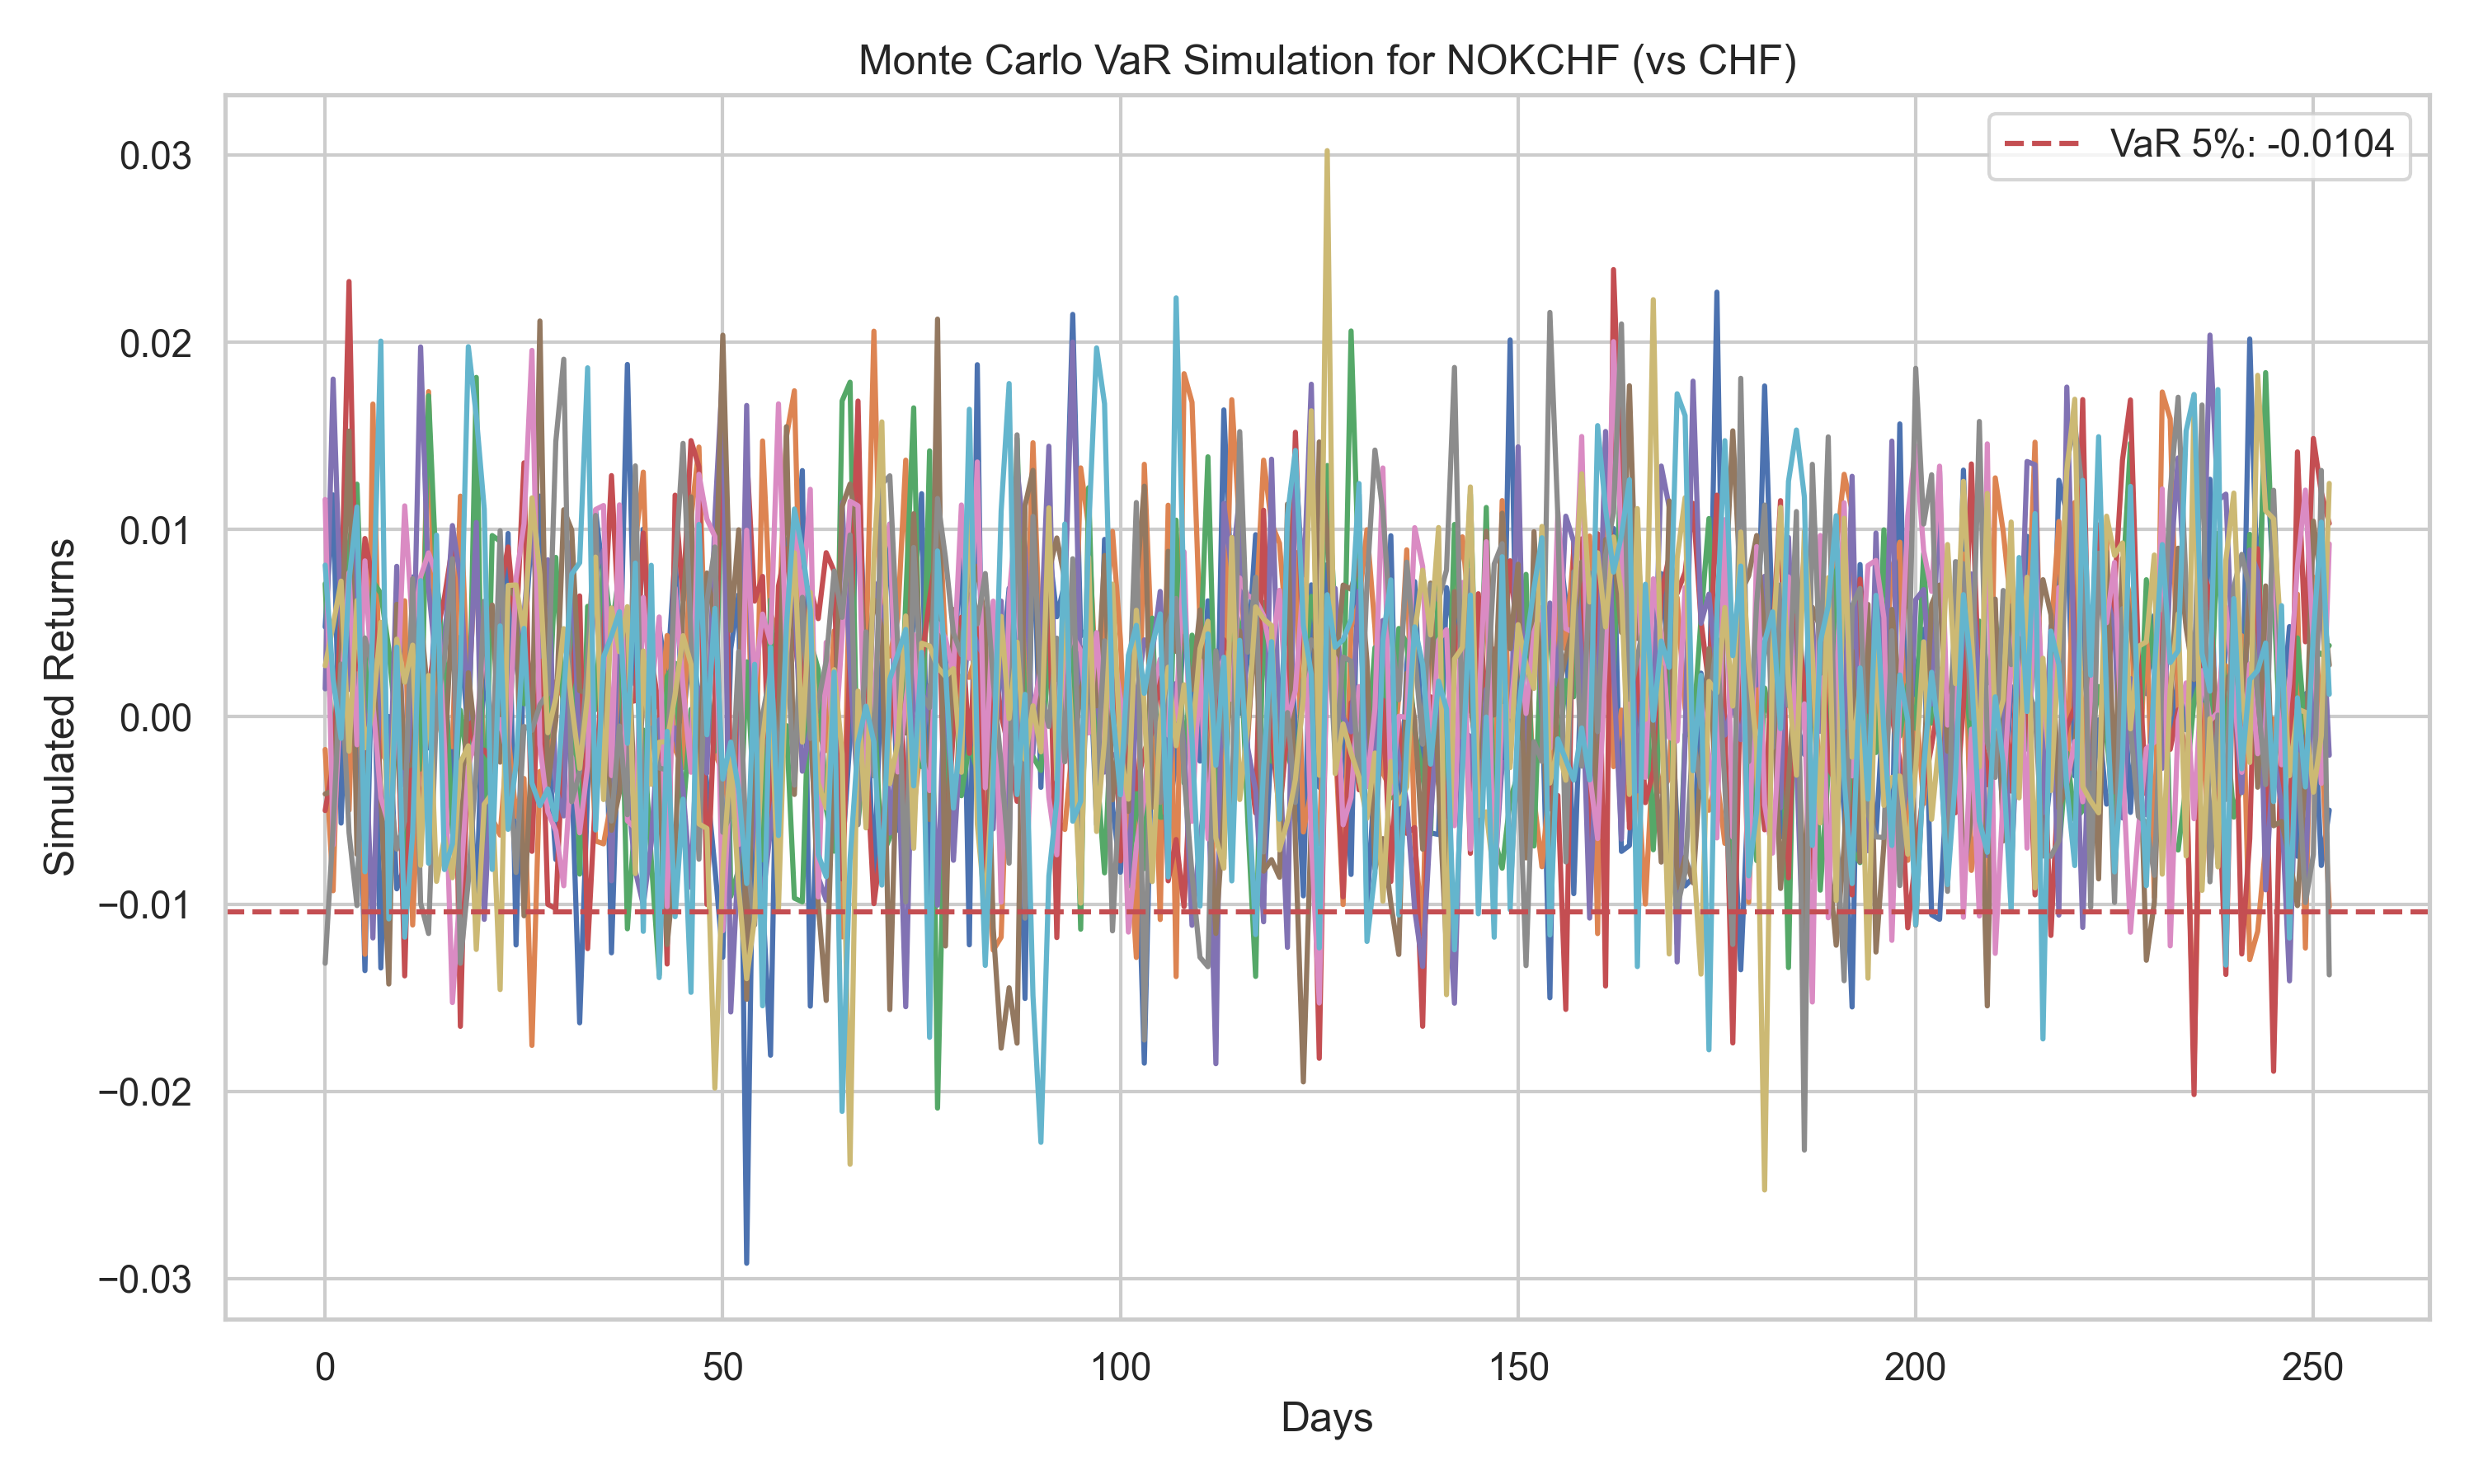
\includegraphics[width=0.48\linewidth]{reports/figures/monte_carlo_var_simulation_NOKCHF_vs_CHF.png} \label{fig:monte_carlo_var_simulation_NOKCHF_vs_CHF}
    \caption{\footnotesize Monte Carlo price siulation (left) and VaR simulation (right) for NOK-CHF.}
\end{figure}
\end{frame}
% ---------------------------------------------------------------------------
\begin{frame}
\frametitle{Main Findings}
\begin{figure}
    \centering  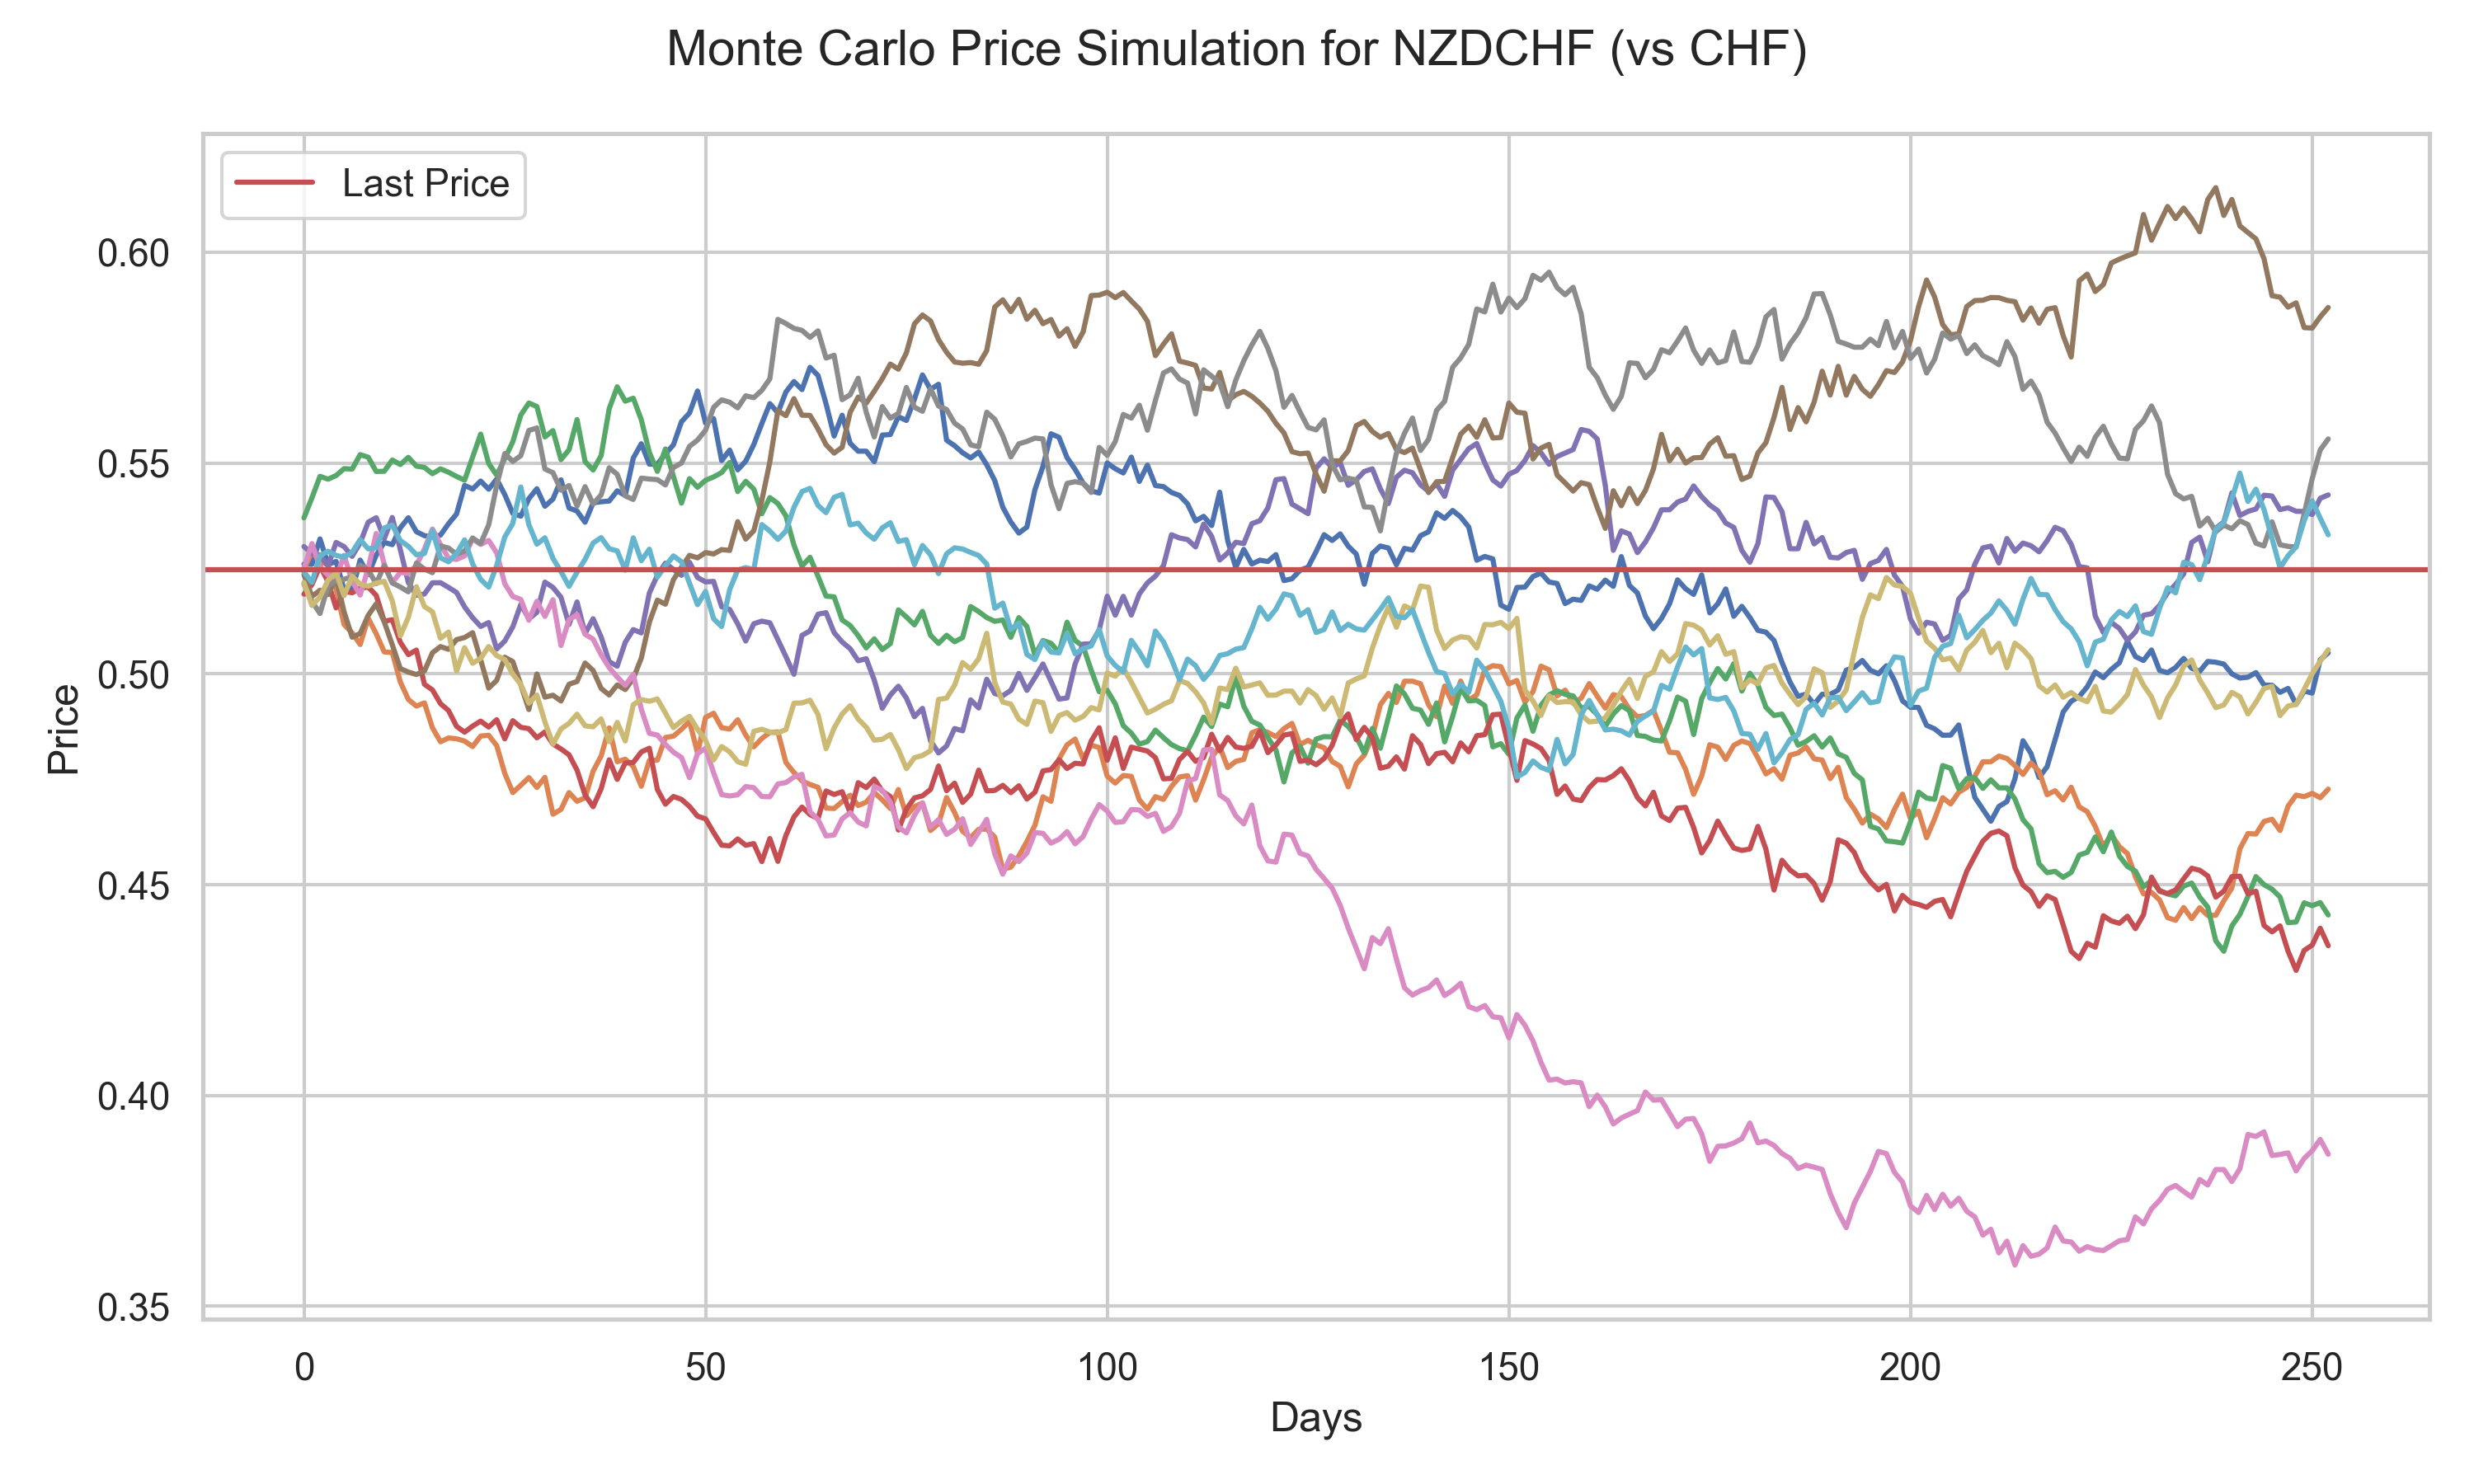
\includegraphics[width=0.48\linewidth]{reports/figures/monte_carlo_price_simulation_NZDCHF_vs_CHF.png}  \label{fig:monte_carlo_price_simulation_NZDCHF_vs_CHF}
    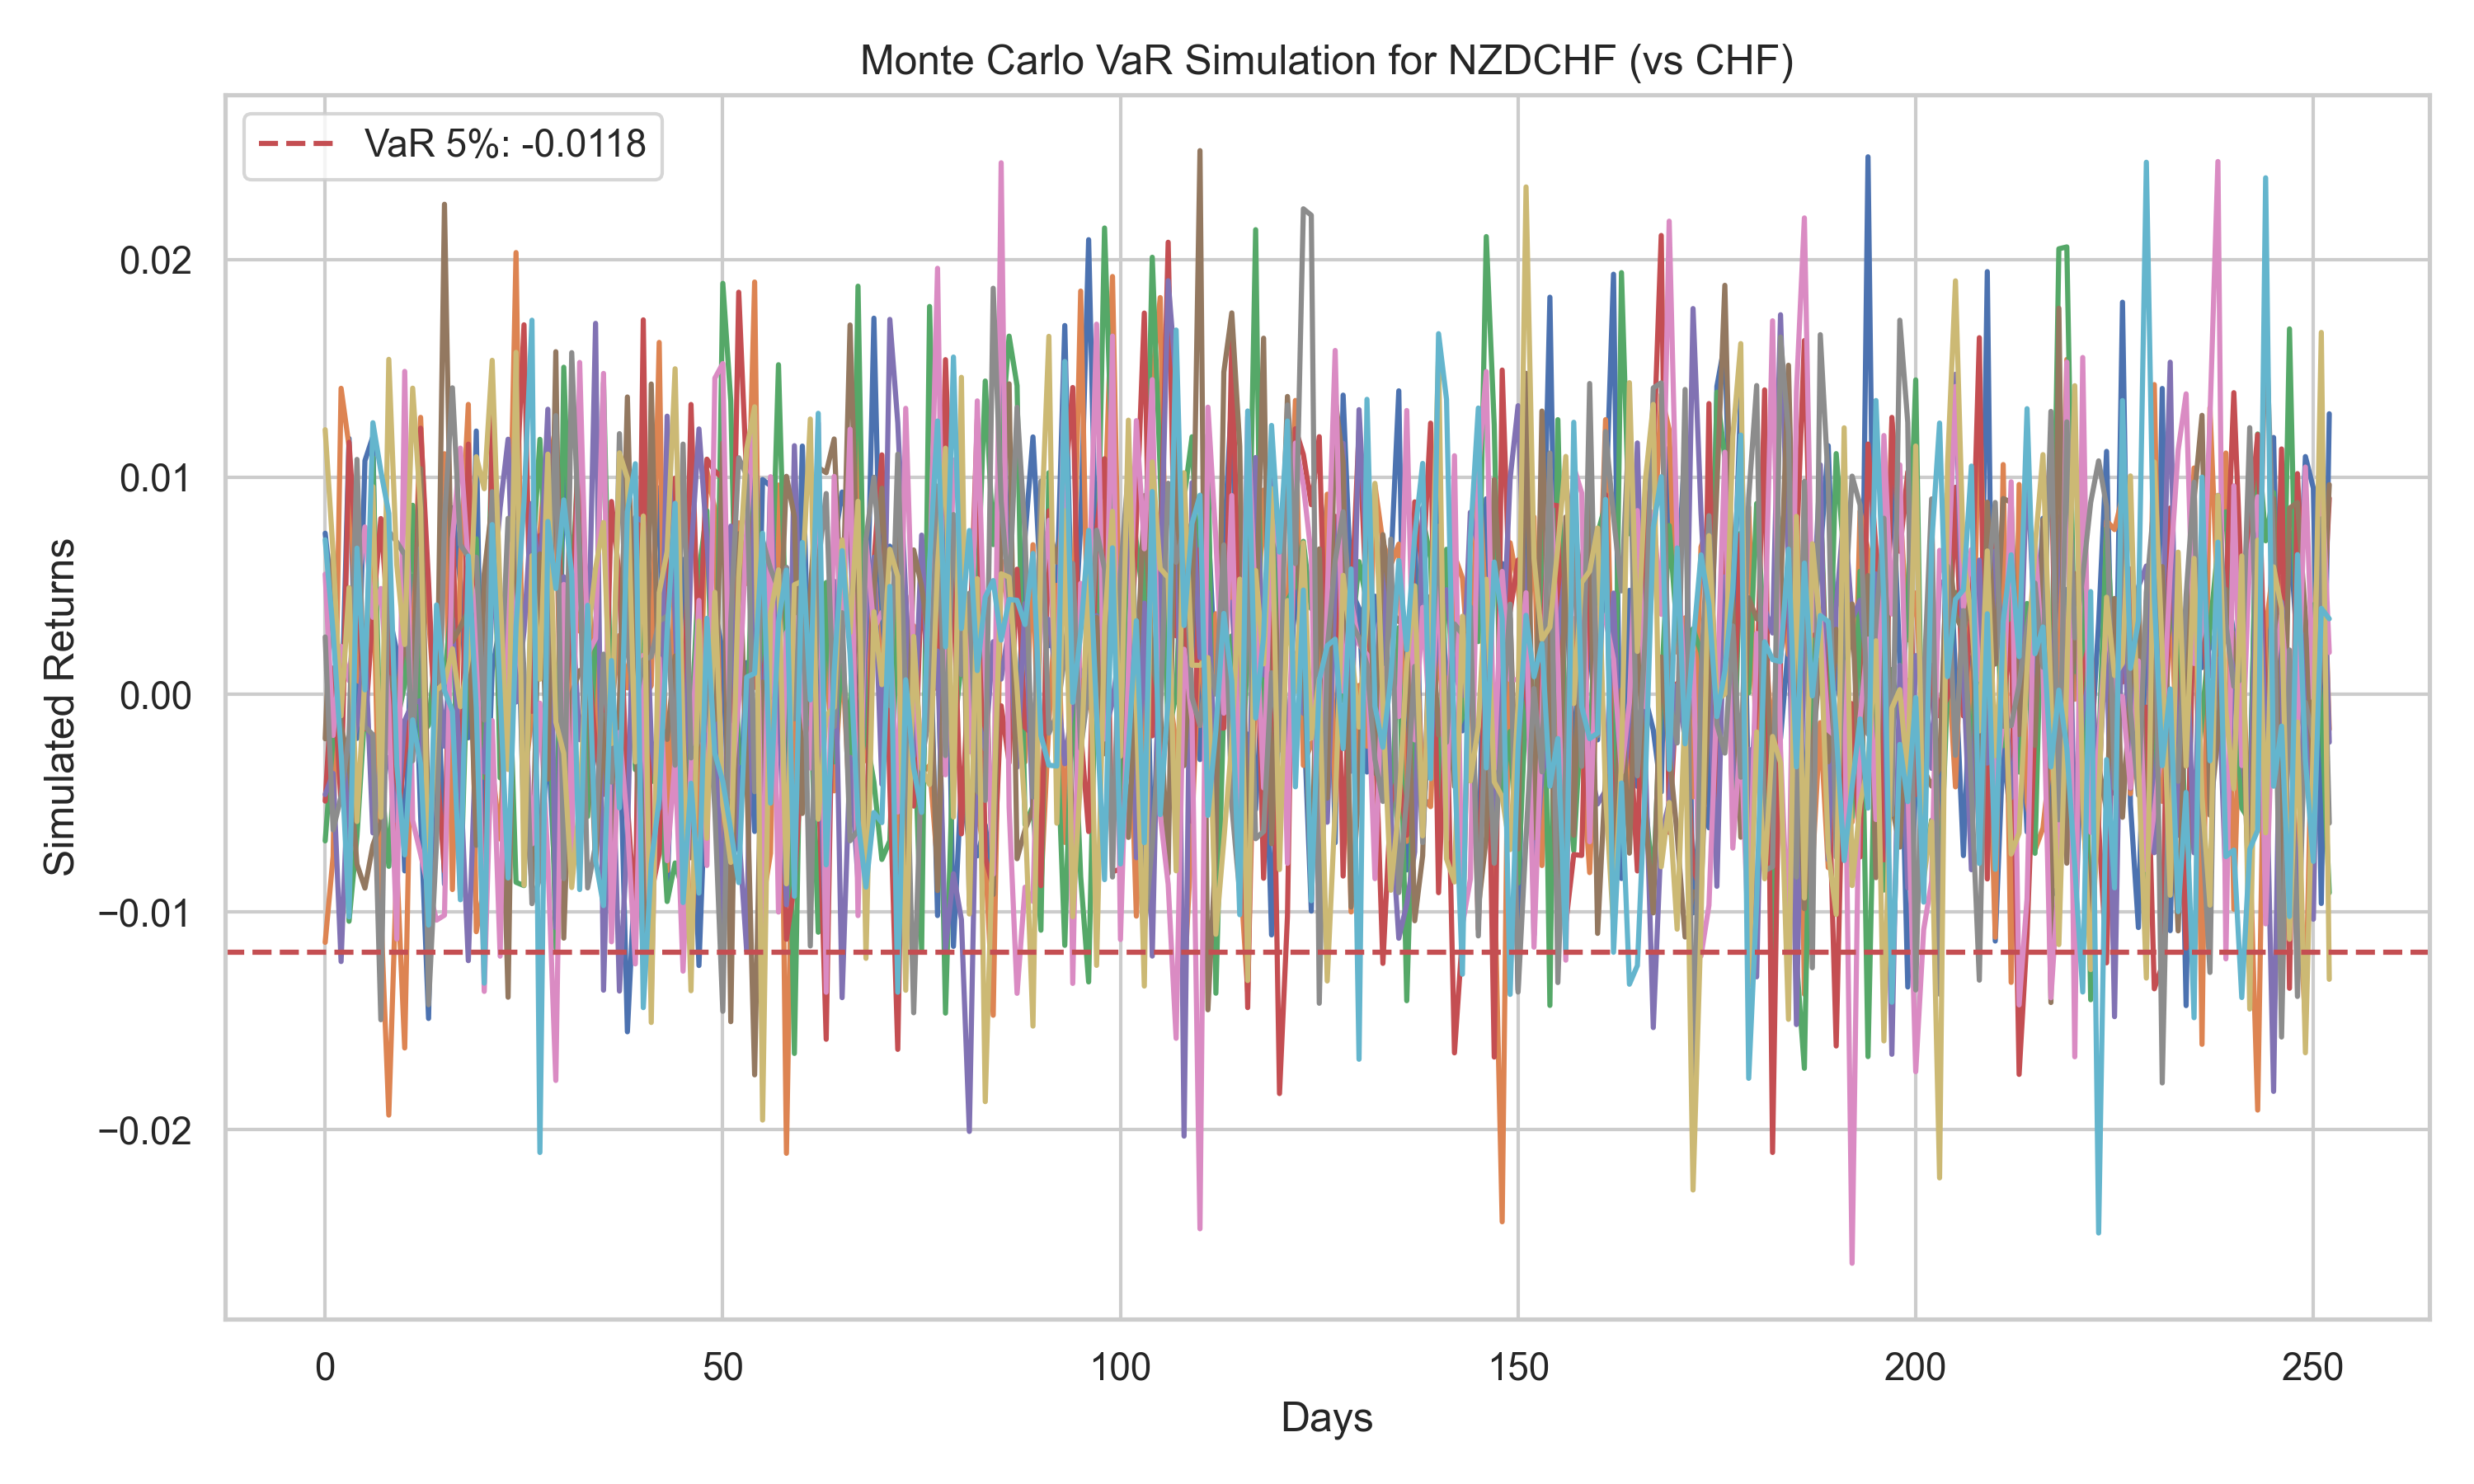
\includegraphics[width=0.48\linewidth]{reports/figures/monte_carlo_var_simulation_NZDCHF_vs_CHF.png}  \label{fig:monte_carlo_var_simulation_NZDCHF_vs_CHF}
    \caption{\footnotesize Monte Carlo price siulation (left) and VaR simulation (right) for NZD-CHF.}
\end{figure}
\begin{figure}
    \centering   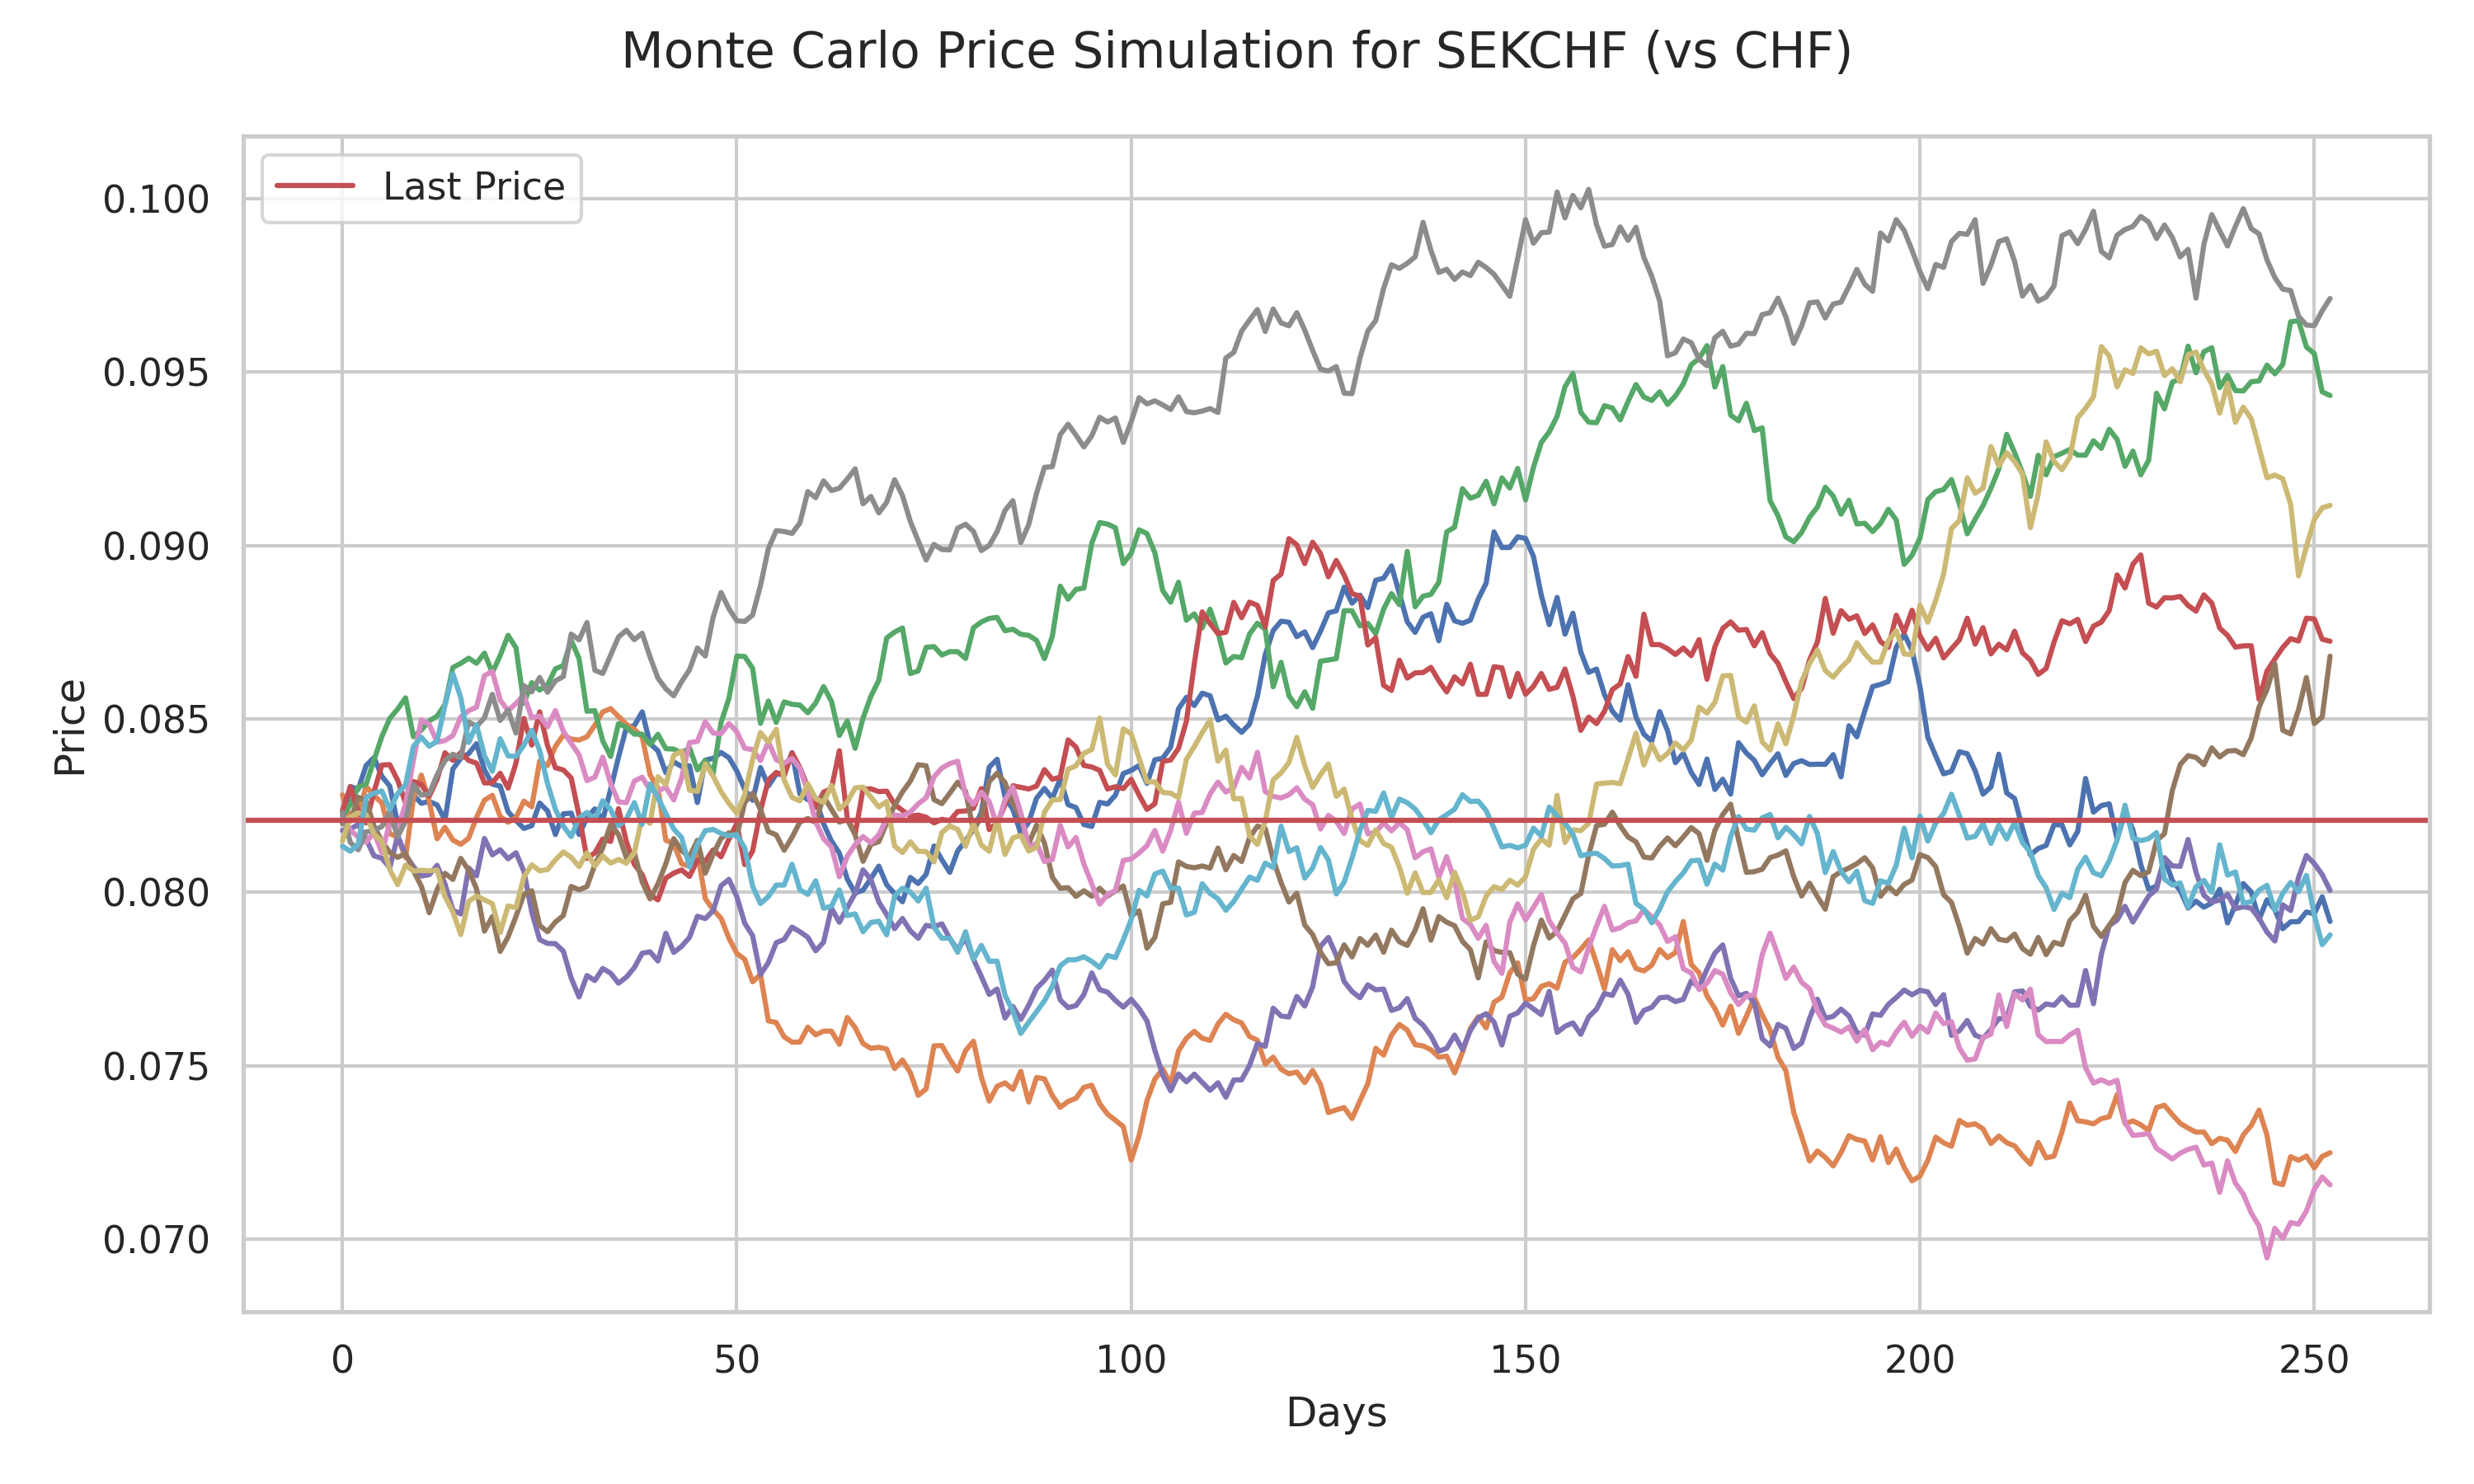
\includegraphics[width=0.48\linewidth]{reports/figures/monte_carlo_price_simulation_SEKCHF_vs_CHF.png} \label{fig:monte_carlo_price_simulation_SEKCHF_vs_CHF}
    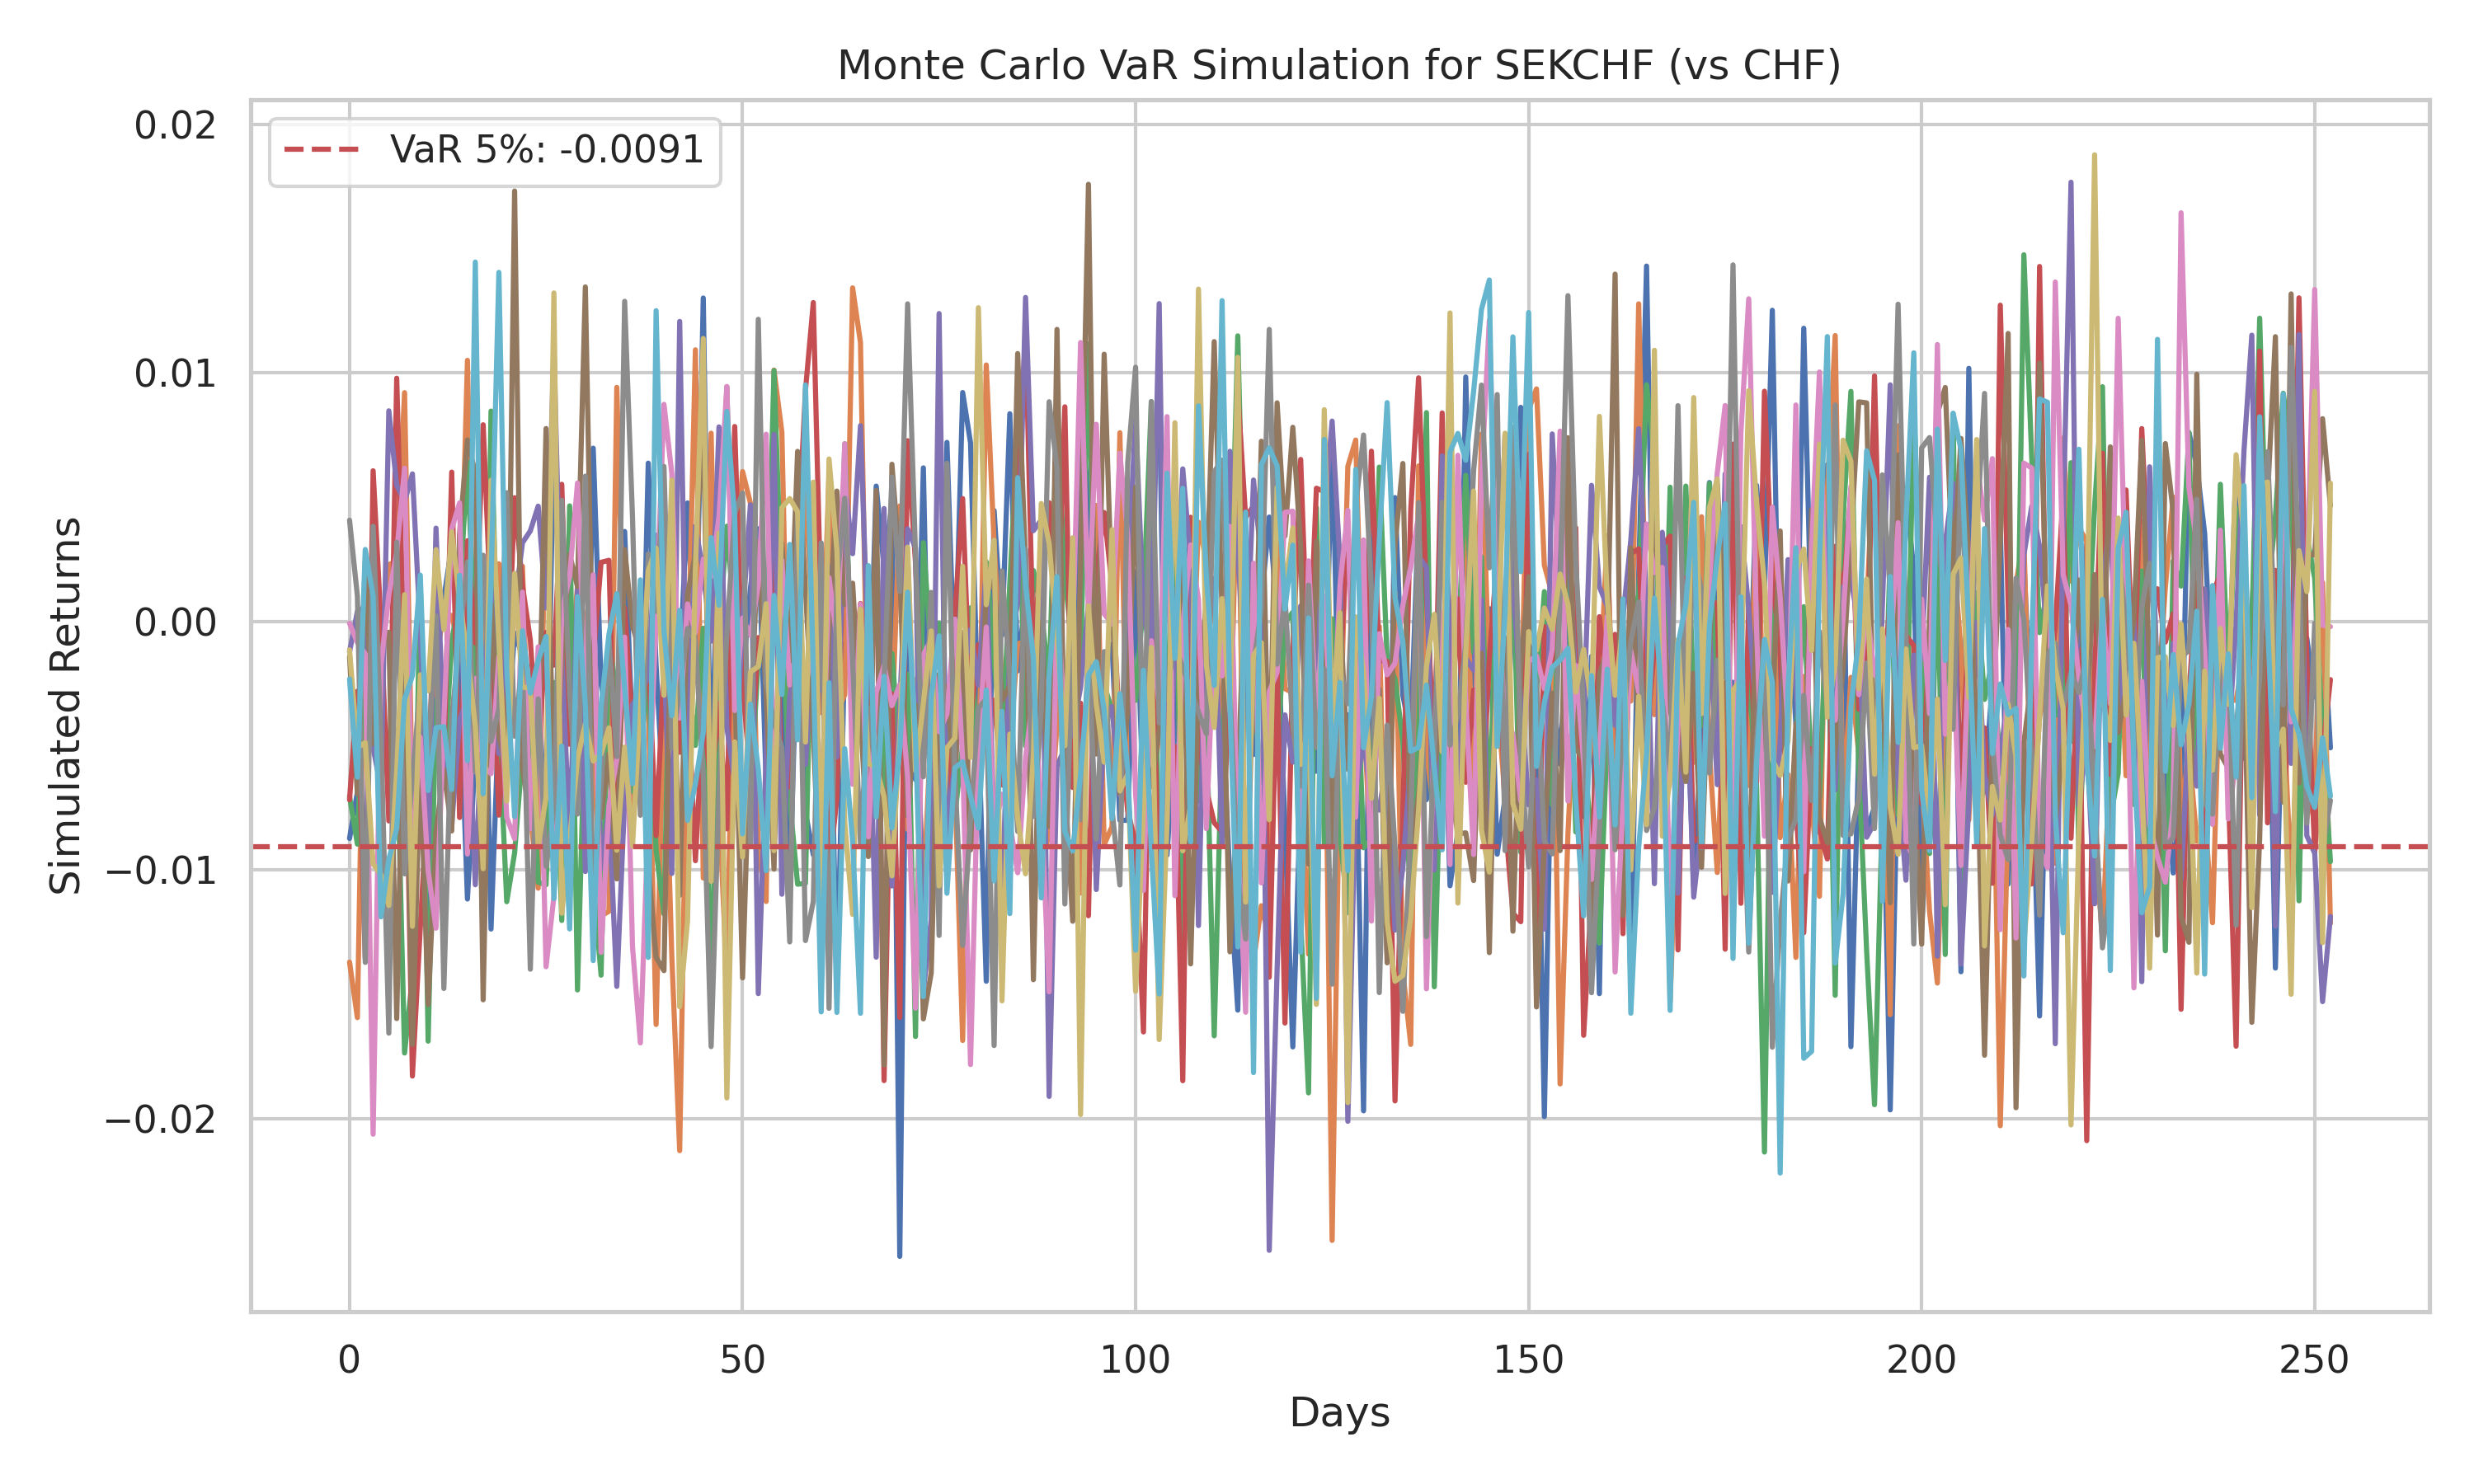
\includegraphics[width=0.48\linewidth]{reports/figures/monte_carlo_var_simulation_SEKCHF_vs_CHF.png} \label{fig:monte_carlo_var_simulation_SEKCHF_vs_CHF}
    \caption{\footnotesize Monte Carlo price siulation (left) and VaR simulation (right) for SEK-CHF.}
\end{figure}
\end{frame}
% ---------------------------------------------------------------------------
\begin{frame}
\frametitle{Main Findings}
\begin{figure}
    \centering  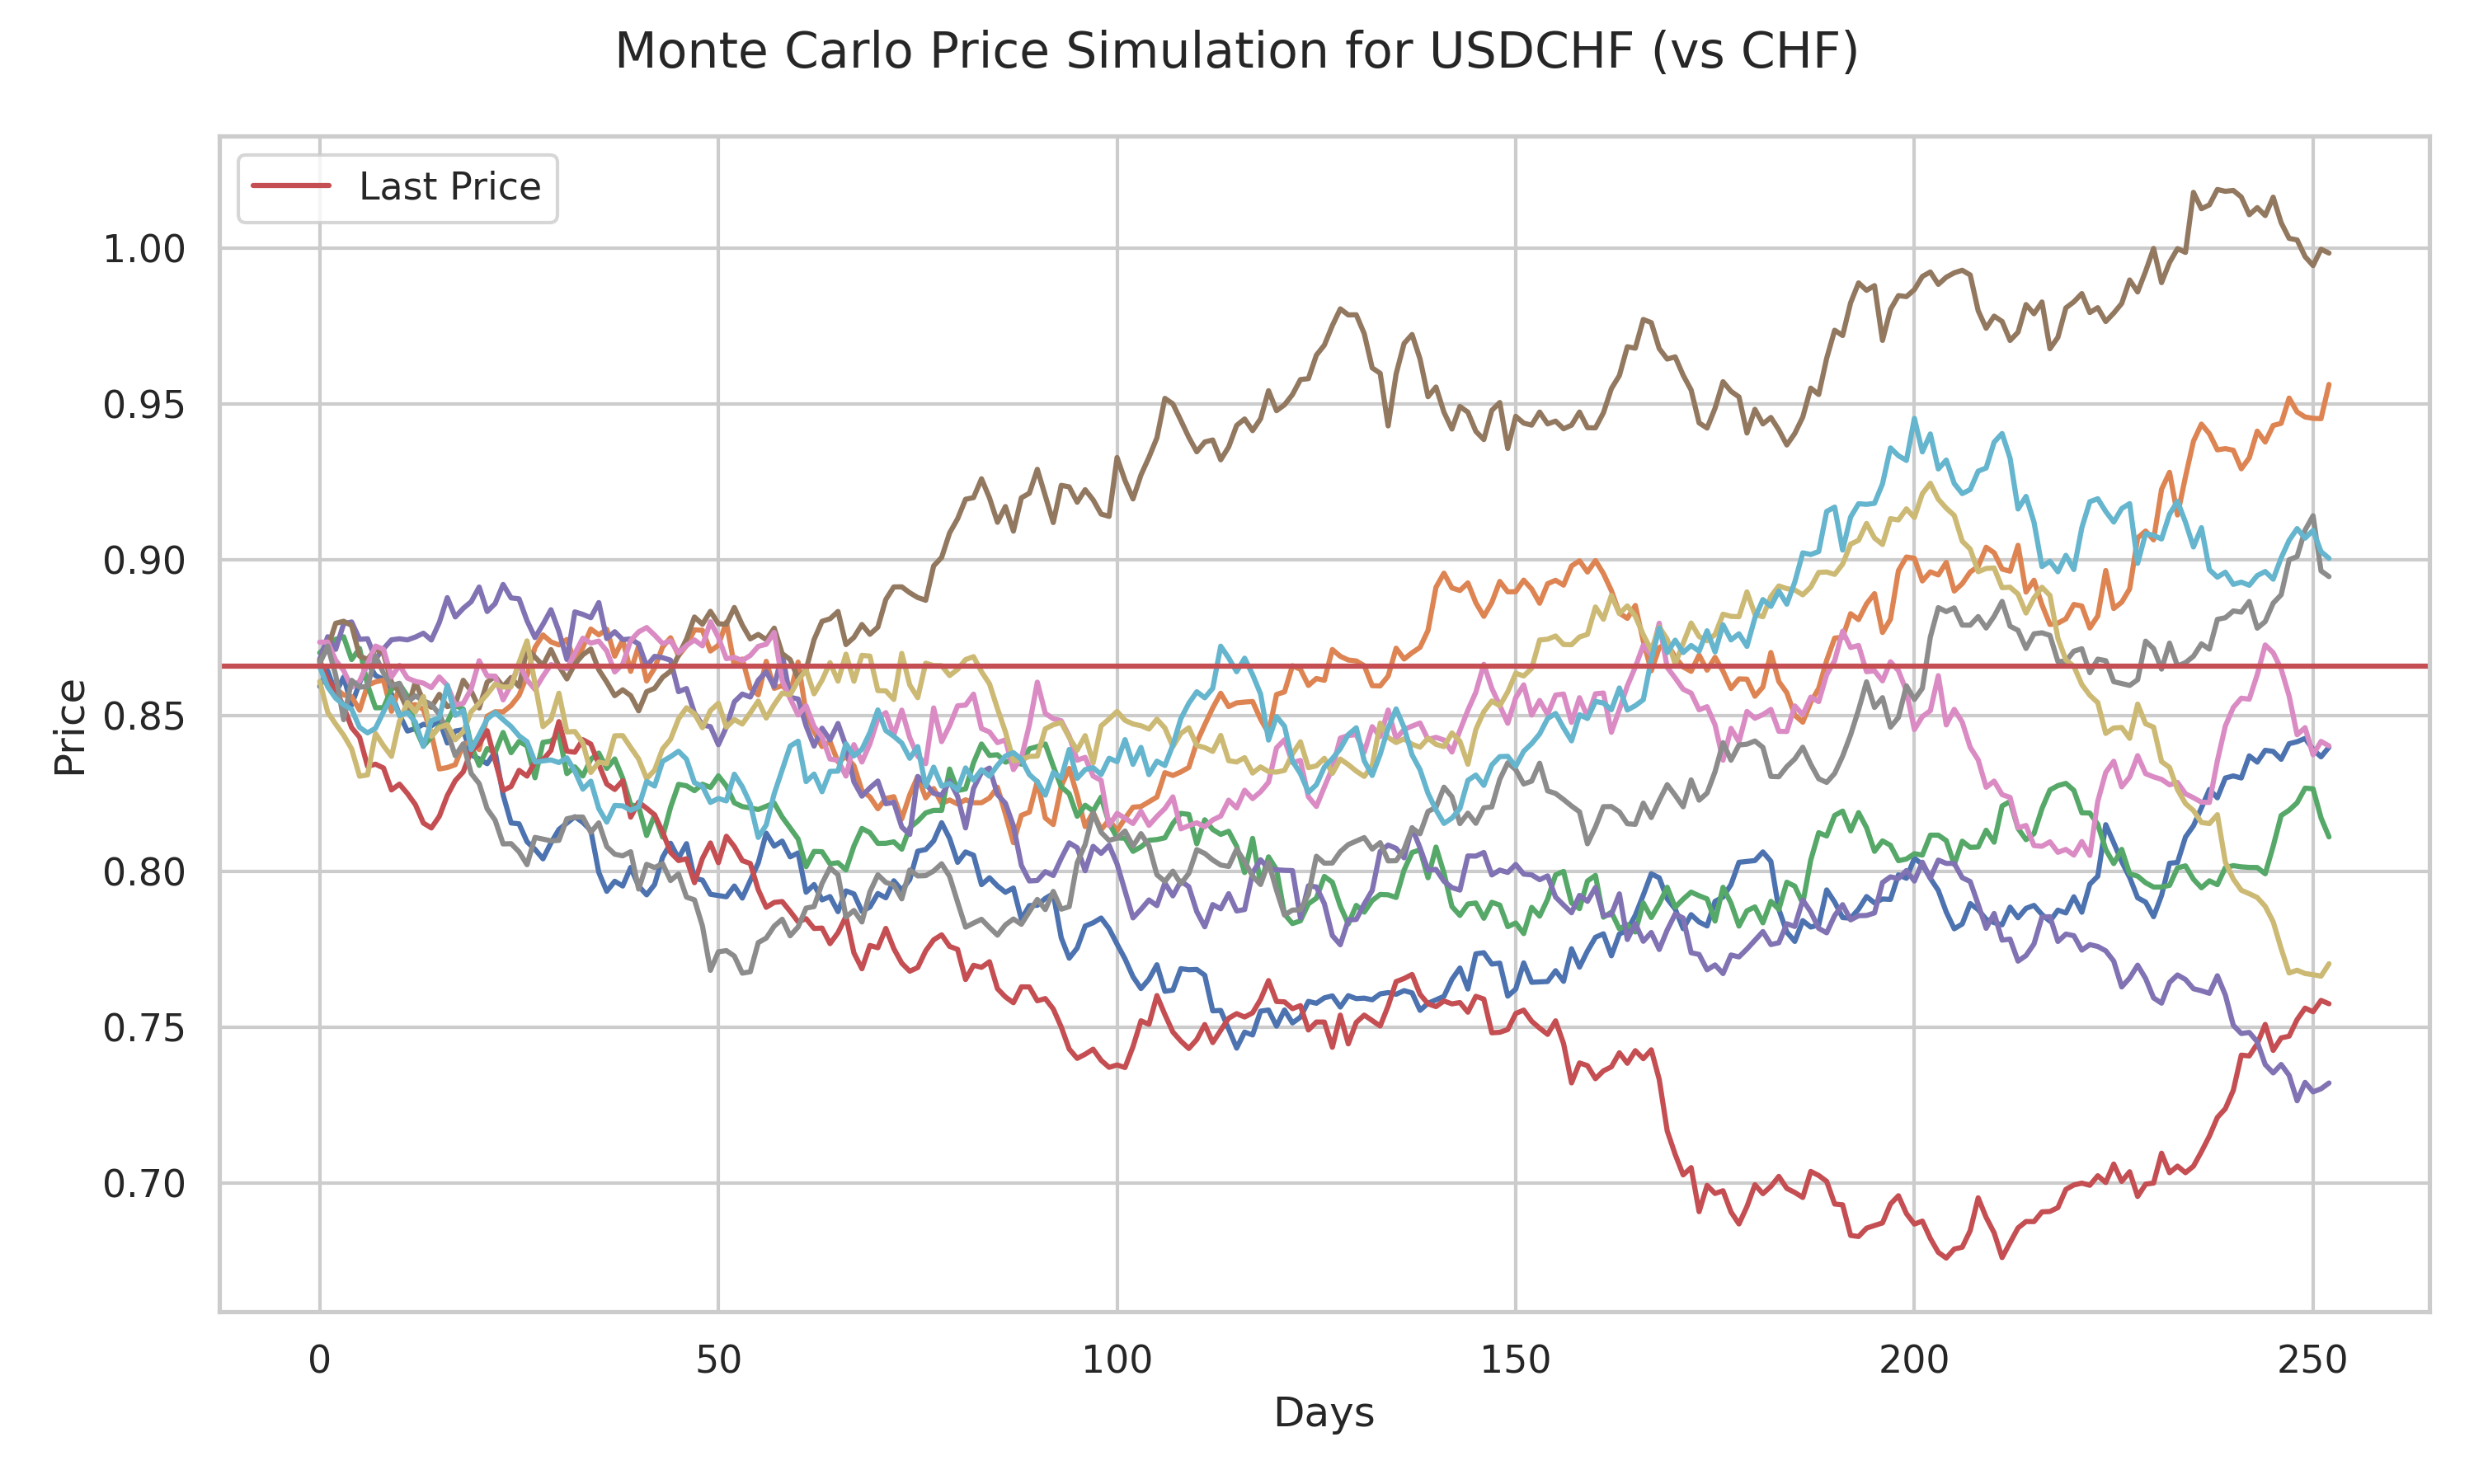
\includegraphics[width=0.48\linewidth]{reports/figures/monte_carlo_price_simulation_USDCHF_vs_CHF.png}  \label{fig:monte_carlo_price_simulation_USDCHF_vs_CHF}
    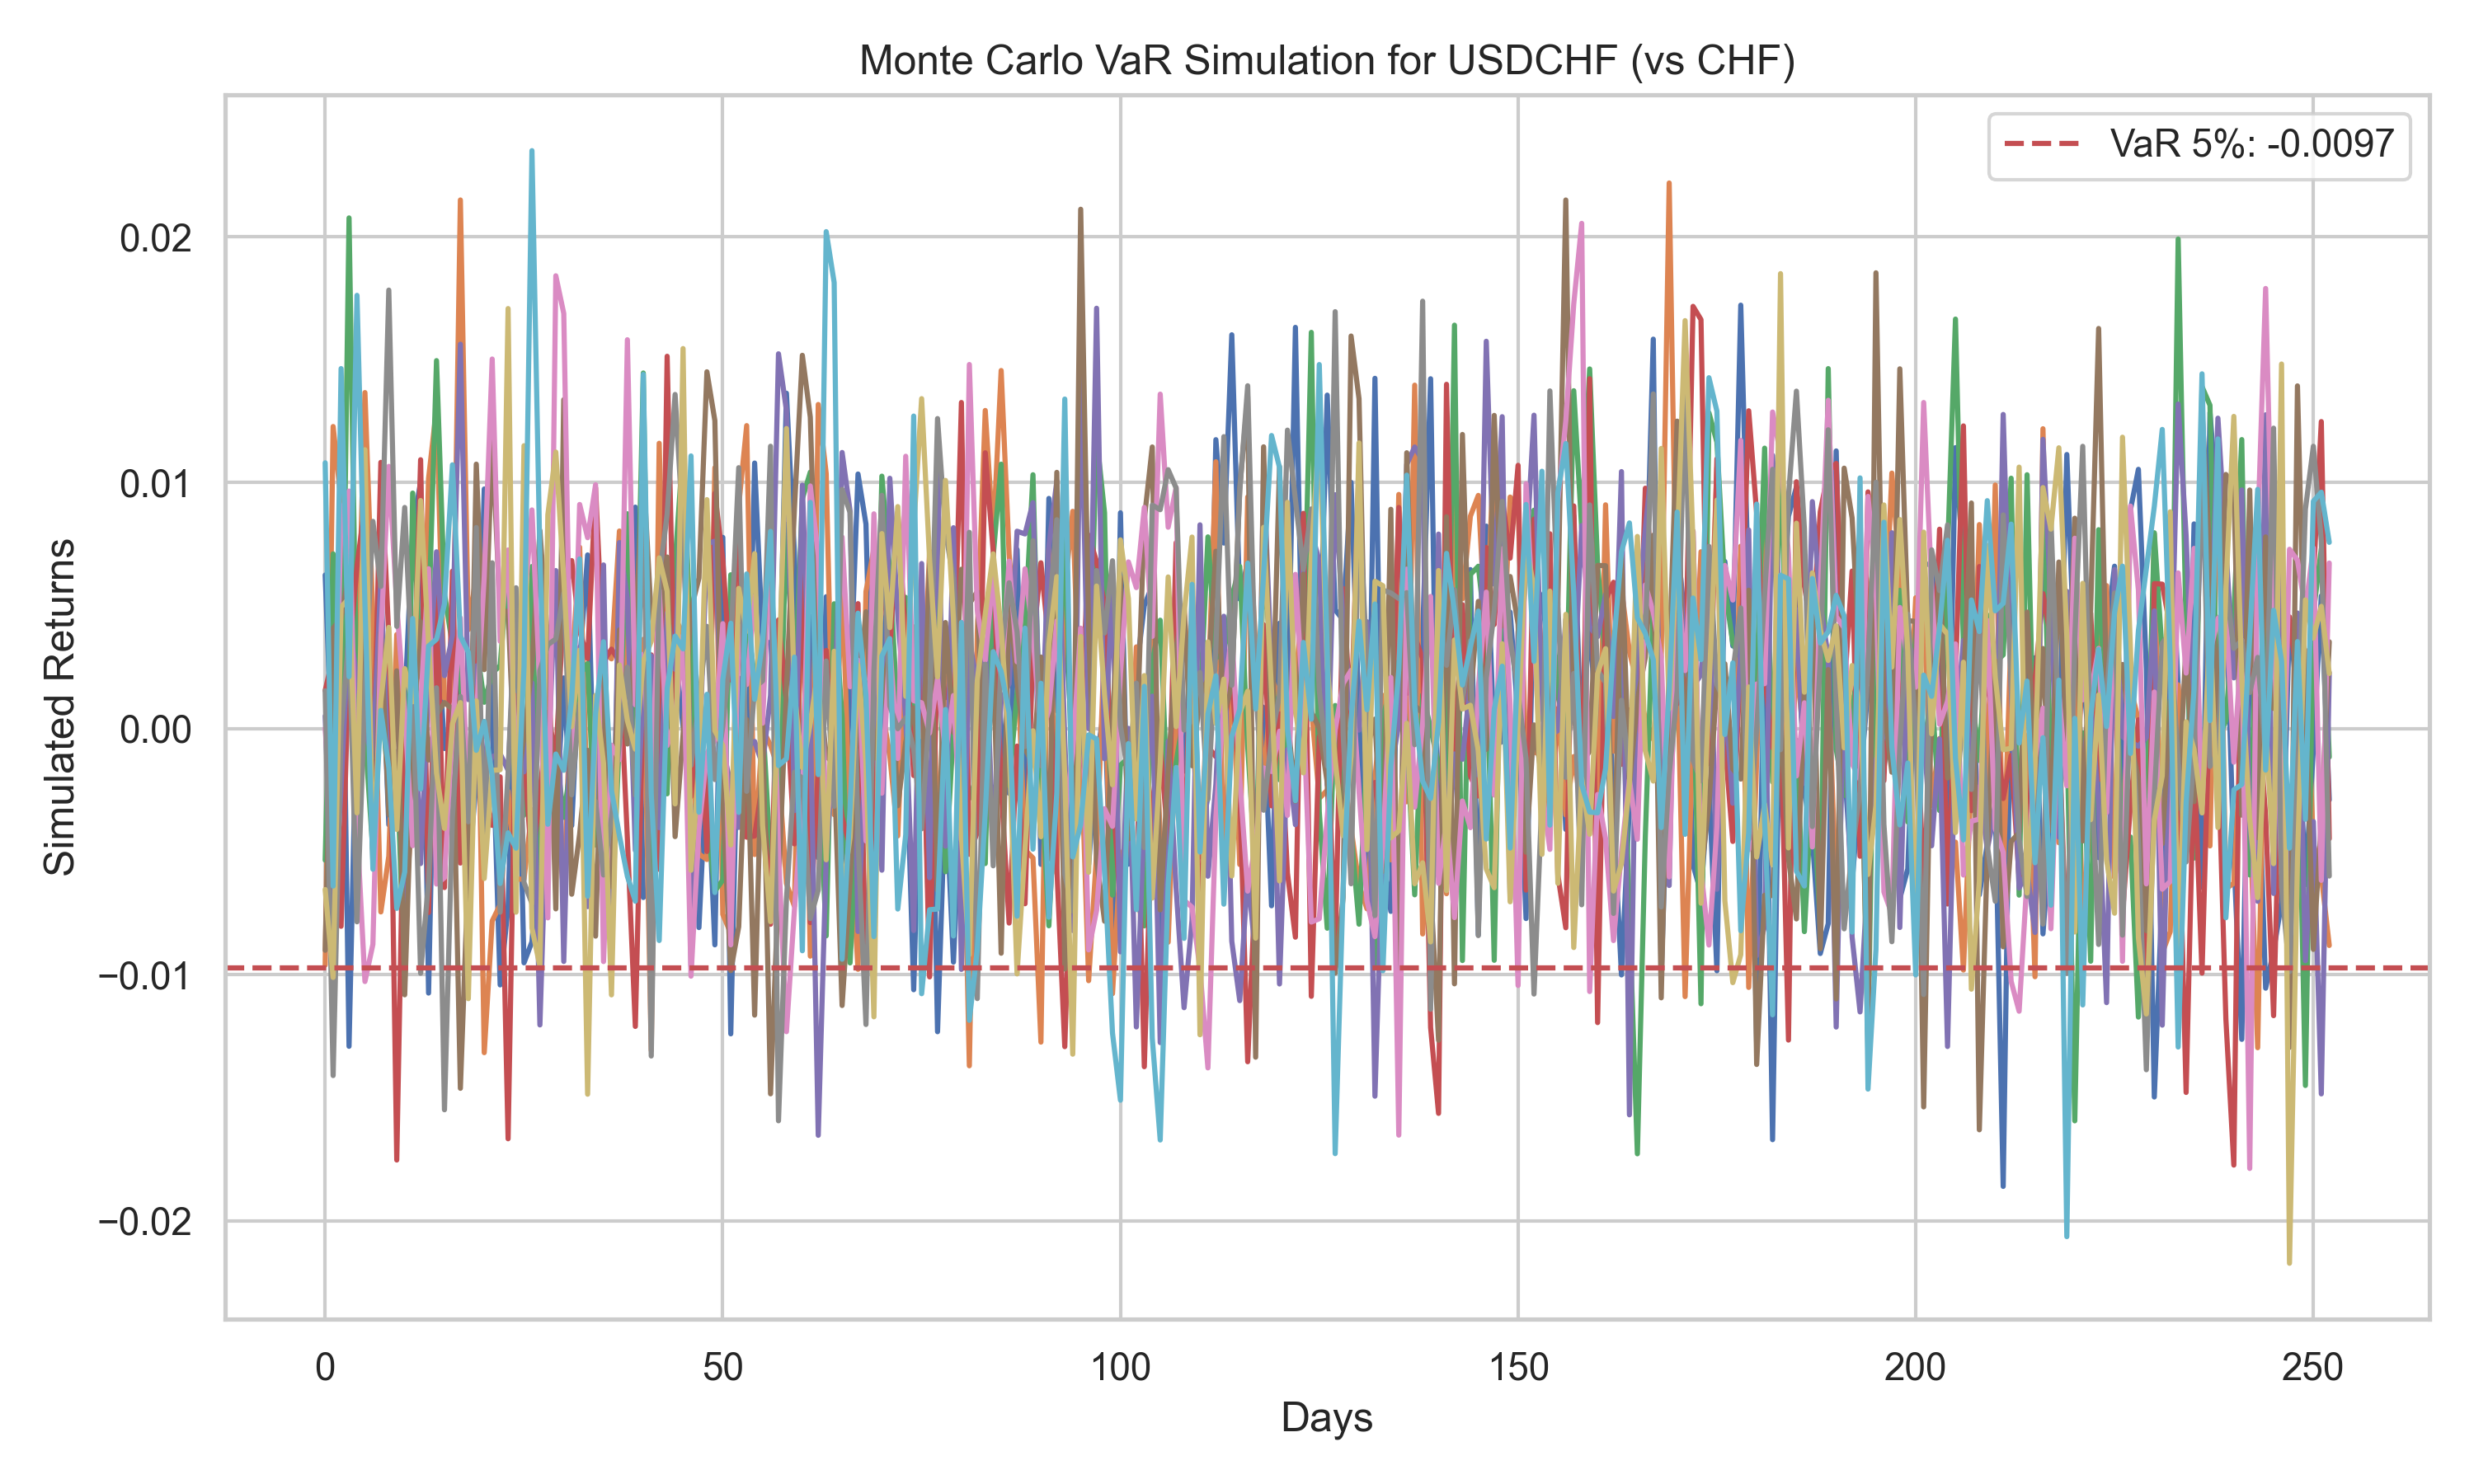
\includegraphics[width=0.49\linewidth]{reports/figures/monte_carlo_var_simulation_USDCHF_vs_CHF.png}  \label{fig:monte_carlo_var_simulation_USDCHF_vs_CHF}
    \caption{\footnotesize Monte Carlo price siulation (left) and VaR simulation (right) for USD-CHF.}
\end{figure}
\end{frame}
% ---------------------------------------------------------------------------
\begin{frame}
\section{Conclusion}
\frametitle{Conclusion}

\end{frame}
% ---------------------------------------------------------------------------
\begin{frame}
\section{References}
\frametitle{References}
\printbibliography
\end{frame}
% ---------------------------------------------------------------------------

\end{document}
